\documentclass[a4paper, 14pt]{extarticle}

% \usepackage[14pt]{extsizes} % чтобы использовать шрифт размером больше 12
\usepackage{cmap} % для кодировки шрифтов в pdf
\usepackage[T2A]{fontenc} % пакет указывает внутреннюю кодировку в системе LaTeX
\usepackage[utf8]{inputenc} % кодировка
\usepackage[english, russian]{babel} % пакет для локализации

\usepackage{graphicx} % для вставки картинок
\usepackage{amssymb,amsfonts,amsmath,amsthm} % математические дополнения от АМС
\usepackage{indentfirst} % отделять первую строку раздела абзацным отступом тоже
\usepackage{makecell} % для создания таблиц
\usepackage{multirow} % для продвинутых таблиц
\usepackage{setspace} % для изменения междустрочного интервала
\usepackage{ulem} % подчеркивания
\usepackage{csvsimple} % для импорта csv - таблиц
\usepackage{siunitx,array,booktabs}
\usepackage[tableposition=top]{caption}
\usepackage{bm}
\usepackage{float}
\usepackage{fancyhdr,fancybox, subcaption}

\usepackage[left=3cm, top=2cm, right=1cm, bottom=2cm, bindingoffset=0cm]{geometry} % настройки полей документа

\pagestyle{plain}
\fancyhead[L]{\thepage}
\renewcommand{\headrulewidth}{0pt}

\addto\captionsrussian{\def\refname{СПИСОК ИСПОЛЬЗОВАННЫХ ИСТОЧНИКОВ}}

\newcommand{\area}{rectangle}
\newcommand{\task}{3_fixes}
\newcommand{\taskNum}{01}

\captionsetup[subfigure]{labelformat=simple, labelsep=colon}
\renewcommand{\thesubfigure}{\alph{subfigure}}



\linespread{1.3} % полуторный интервал

\begin{document} % начало документа

\begin{titlepage}
\normalsize
\thispagestyle{empty}
\begin{center}
\small{\textbf{Министерство образования и науки Российской Федерации}}
\\[-0.3em]
\small{\textbf{Федеральное государственное бюджетное образовательное учреждение}} 
\\[-0.3em]
\small{\textbf{высшего образования}} 
\\[-0.3em]
\small{\textbf{<<Московский государственный технический университет}} 
\\[-0.3em]
\small{\textbf{имени Н.Э.Баумана}} 
\\[-0.3em]
\small{\textbf{(национальный исследовательский университет)>>}} 
\\[-0.3em]
\small{\textbf{(МГТУ им. Н.Э.Баумана)}}
\\[-0.7em]
\rule{\textwidth}{4 pt}
\end{center}
\medskip
\small{ФАКУЛЬТЕТ <<Фундаментальные науки>>}
\\[2em]
\small{КАФЕДРА <<Прикладная математика>>} \\
\begin{center}
\Large{\textbf{РАСЧЕТНО-ПОЯСНИТЕЛЬНАЯ ЗАПИСКА}}
\\[\bigskipamount]
\large{\textit{\textbf{К ВЫПУСКНОЙ КВАЛИФИКАЦИОННОЙ РАБОТЕ}}}
\\[\bigskipamount]
\Large{\textbf{НА ТЕМУ:}}
\\[\medskipamount]
\large{<<Применение различных вариантов метода декомпозиции области для численного решения задач деформирования упругих тел>>}
\end{center}
\vspace{2em}
Студент ФН2-42М \hspace{17.7em}  $\underset{\text{\footnotesize{(Подпись, дата)}}}{\rule{7em}{1 pt}}$ \ М.В. Матвеев
\\[2em]
Руководитель ВКР \hspace{17em} $\underset{\text{\footnotesize{(Подпись, дата)}}}{\rule{7em}{1 pt}}$ \ А.С. Родин
\\[2em]
Консультант \hspace{20em} $\underset{\text{\footnotesize{(Подпись, дата)}}}{\rule{7em}{1 pt}}$ \ \rule{6.5em}{1 pt}
\\[2em]
Консультант \hspace{20em} $\underset{\text{\footnotesize{(Подпись, дата)}}}{\rule{7em}{1 pt}}$ \ \rule{6.5em}{1 pt}
\\[2em]
Нормоконтролер \hspace{18.2em}  $\underset{\text{\footnotesize{(Подпись, дата)}}}{\rule{7em}{1 pt}}$ \ М.М. Лукашин
\vspace{1em}
\begin{center}
2021 г.
\end{center}
\end{titlepage}

\newpage

\begin{center}
\section*{\centering РЕФЕРАТ}
\end{center}
\setcounter{page}{2}
\addcontentsline{toc}{section}{РЕФЕРАТ}

Расчётно-пояснительная записка 63 с., 20 рис., 27 табл., 15 источников.

ДЕФОРМИРОВАНИЕ ТЕЛ, МЕТОДЫ ДЕКОМПОЗИЦИИ, МЕТОДЫ ШВАРЦА, МУЛЬТИПЛИКАТИВНЫЕ МЕТОДЫ, АДДИТИВНЫЕ МЕТОДЫ, ДВУХУРОВНЕВЫЕ МЕТОДЫ

При численном решении задач деформирования упругих тел в виде дифференциальных уравнений в частных производных, чаще всего матрица получившейся системы линейных уравнений получается сильно разреженной. В таком случае лучше всего использовать итерационные методы решения системы. Одним из эффективных способов решения подобной задачи является метод декомпозиции области.

Цель работы - применить методы декомпозиции области для решения задач деформирования упругих тел и исследовать сходимость разных вариаций методов декомпозиции области.

Результаты, полученные при решении ряда тестовых задач, показывают, что двухуровневый аддитивный метод Шварца выигрывает у мультипликативного и аддитивного методов Шварца по нескольким параметрам: во-первых, локальные задачи в каждой из подобластей решаются независимо друг от друга, количество итераций не зависит практически ни от изменения шага сетки, ни от изменения количества подобластей, на которое разбивается исходная область.

\newpage

\renewcommand*\contentsname{\begin{center}СОДЕРЖАНИЕ\end{center}}
	
\tableofcontents

\newpage

\begin{center}
\section*{\centering ВВЕДЕНИЕ}
\end{center}
\addcontentsline{toc}{section}{ВВЕДЕНИЕ}

При численном решении задач деформирования упругих тел в виде дифференциальных уравнений в частных производных, чаще всего матрица получившейся системы линейных уравнений получается сильно разреженной. Лучше всего в таком случае использовать итерационные методы решения системы. 

Одним из эффективных способов решения подобной задачи является метод декомпозиции области. Благодаря ему можно свести решение задачи в большой области к решению множества локальных задач в подобластях меньшего размера, но с учётом дополнительных итераций внутри области. За счёт количества подобластей размеры полученных систем линейных уравнений для каждой из локальных задач остаются приемлемыми. На данный момент существуют разные методы декомпозиции области. У некоторых методов общее количество итераций не зависит от шага выбранной сетки для области, но, при этом, довольно сильно зависит от количества подобластей. Существуют также методы, где данная проблема устранена, и количество итераций кардинально не зависит ни от шага сетки, ни от количества вводимых подобластей. Локальные задачи, в зависимости от выбранного метода, могут решаться как последовательно, так и независимо друг от друга.

Целью работы является применение методов декомпозиции области для решения задач деформирования упругих тел и исследование сходимости для разных вариантов методов декомпозиции области.

Для достижения поставленной цели решены следующие задачи:
\begin{itemize}
\item[-]рассмотрение модели упругого материала;
\item[-]исследование мультипликативного, аддитивного и двухуровневого аддитивного методов Шварца;
\item[-]реализация мультипликативного, аддитивного и двухуровневого аддитивного методов Шварца в виде программы для моделей упругого материала;
\item[-]проведение серии расчётов для ряда тестовых задач;
\item[-]исследование сходимости путём сравнения количества итераций для мультипликативного, аддитивного и двухуровневого аддитивного методов Шварца;
\item[-]изучение скорости роста итераций и временных затрат при решении задачи методом сопряженных градиентов.
\end{itemize}

\newpage
 
\section{Математическая модель}

\subsection{Постановка задачи}

Для решения общей задачи по нахождению деформаций и напряжений в деформируемом теле, занимающем область $G$ с границей $\partial \, G$, необходимо использовать следующие соотношения \cite{3}:

\begin{itemize}

\item уравнение равновесия
\begin{equation}
L \mathbf{u} = - \triangledown \bm{\sigma(u)} = \mathbf{f(x)}
\end{equation}

\item кинематические граничные условия
\begin{equation}
\bm{u(x)} = u_0, \ x \in \partial \, G_D,
\end{equation}

\item силовые граничные условия
\begin{equation}
\bm{\sigma}\mathbf{(u) \cdot n} = \mathbf{p(x)}, \ x \in \partial \, G_N,
\end{equation}

\item соотношение Коши для тензора полных деформаций
\begin{equation}
\bm{\varepsilon(u)}=\dfrac{1}{2}(\nabla u + (\nabla u)^T,
\end{equation}

\item уравнение для тензора напряжений
\begin{equation}
\bm{\sigma(u)} = \mathbf{C \cdot} \bm{\varepsilon}\mathbf{(u)},
\end{equation}
\end{itemize}

где $\mathbf{u(x)}$ - вектор перемещений, $\mathbf{f(x)}$ - вектор массовых сил, $\partial \, G_D$ - участок границы области $G$, на котором заданы кинематические условия, $\partial \, G_N$ - участок границы области $G$, на котором заданы силовые условия, $\mathbf{p(x)}$ - вектор внешней нагрузки, действующей на участке $\partial \, G_N$, $\mathbf{C}$ - тензор упругих коэффициентов. 

\newpage

\subsection{Методы Шварца}

Решить данную задачу можно с помощью методов декомпозиции области. Методы декомпозиции области области бывают двух видов: с перекрытием и без перекрытия подобластей. Один из вариантов метода декомпозиции области с перекрытием подобластей называется методом Шварца.

Рассмотрим классическую задачу метода Шварца для двух подобластей $\left[3\right]$: имеется сложная область $\Omega$, состоящая из объединения двух простых областей (круга $\Omega_1$ и прямоугольника $\Omega_2$). Рассмотрим уравнение, цель которого найти перемещения $u: \Omega \rightarrow \mathbb{R}$ при условии, что
\begin{equation*}
\begin{array}{rl}
-\bigtriangleup \!(u) = f, & u \in \Omega \\
u = 0, & u \in \partial \Omega
\end{array}
\end{equation*}

\begin{figure}[h]
\center{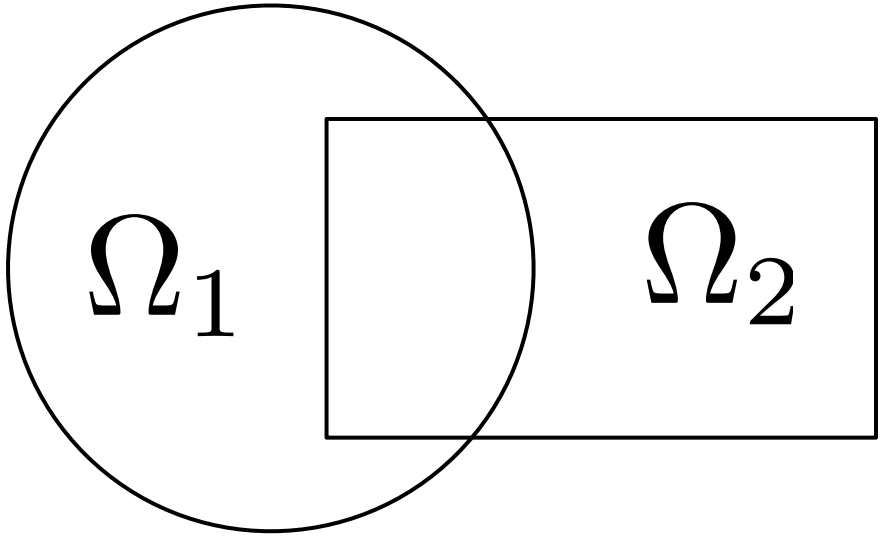
\includegraphics[scale=0.2]{img/simple_domains.png}}
\caption{Сложная область, получившаяся из объединения двух простых областей}
\label{fig:image_01}
\end{figure}

Классический метод Шварца это итерационный метод, основанный на решении задач меньшего масштаба в подобластях $\Omega_1$ и $\Omega_2$. Один шаг итерационного процесса обновления результатов $u^n \rightarrow u^{n+1}$:
\begin{eqnarray*}
-\bigtriangleup \! (u^{n+1}) = f, & u \in \Omega_1 \\
u^{n+1} = 0, & u \in \partial \Omega_1 \cap \partial \Omega \\
u^{n+1} = u^n, & u \in \partial \Omega_1 \cap \bar{\Omega_2}
\end{eqnarray*}
\begin{eqnarray*}
-\bigtriangleup \! (u^{n+1}) = f, & u \in \Omega_2 \\
u^{n+1} = 0, & u \in \partial \Omega_2 \cap \partial \Omega \\
u^{n+1} = u^n, & u \in \partial \Omega_2 \cap \bar{\Omega_1}
\end{eqnarray*}

Рассмотрим случай для произвольной области и произвольного числа подобластей, представим область $G$ в виде объединения конечного числа подобластей $G = \bigcup_{i=1}^{M} G_i$ с конечным числом границ $\partial G_1, \ldots, \partial G_M$, где M - число подобластей. Данные подобласти пересекаются, что требует ввода дополнительных обозначений для границ, возникающих после декомпозиции областей: $\Gamma = \bigcup_{i=1}^{M} \Gamma_i$. 

Выберем начальное приближение для перемещений, удовлетворяющее граничным условиям (ссылка здесь). Алгоритм из классического метода Шварца можно оптимизировать для большего числа подобластей:
\begin{equation*}
\begin{array}{rl}
-\bigtriangleup \! (u^{n+\frac{i}{M}}) = f(x), & x \in G_i \\
\sigma(u^{n+\frac{i}{M}}) \cdot n = p(x), & x \in \partial G_N \cap \partial G_i \\
u^{n+\frac{i}{M}}(x) = 0, & x \in \partial G_D \cap \partial G_i \\ 
u^{n+\frac{i}{M}}(x) = u^{n+\frac{(i - 1)}{M}}(x), & x \in G \setminus ((G_i \setminus \partial G_i) \cap (\partial G_N \cup \partial G_i))
\end{array}
\end{equation*}

Данный алгоритм Шварца называют мультипликативным, он последовательный и решение на каждой подобласти зависит от решения на предыдущей подобласти (или от решения на предыдущей итерации, если речь идёт о первой подобласти для итерации).

Существует также другой вариант метода Шварца, основанный на решении локальных задач для каждой подобласти без зависимости от соседних подобластей:
\begin{equation*}
\begin{array}{rl}
-\bigtriangleup \! (u^{n+\frac{i}{M}}) = f(x), & x \in G_i \\
\sigma(u^{n+\frac{i}{M}}) \cdot n = p(x), & x \in \partial G_N \cap \partial G_i \\
u^{n+\frac{i}{M}}(x) = 0, & x \in \partial G_D \cap \partial G_i \\ 
u^{n+1}(x) = u^{n}(x), & x \in G \setminus ((G_i \setminus \partial G_i) \cap (\partial G_N \cup \partial G_i))
\end{array}
\end{equation*}

Этот метод называется аддитивный метод Шварца. В конце каждой итерации решение вычисляется по формуле 
\begin{equation*}
u^{n+1} = u^{n} + \alpha \sum_{i=1}^{M} (u_i^{n+1} - u^{n}),
\end{equation*}
где коэффициент $\alpha$ - параметр скорости сходимости итерационного процесса. 

\newpage

\section{Численная модель}

\subsection{Теоретические сведения}

\subsubsection{Линейные треугольные элементы}

Линейный треугольный элемент представляет из себя треугольник с тремя узлами $i, j, k$ по одному на каждую из трёх вершин в плоскости $(x, y)$. Дальнейшая нумерация узлов проводится против часовой стрелки. Компоненты элементного вектора узловых перемещений обозначим как $\left( u_i, u_j, u_k \right)$, декартовы координаты узлов - как $(x_i, y_i), (x_j, y_j), (x_k, y_k)$. 

\begin{figure}[h]
\center{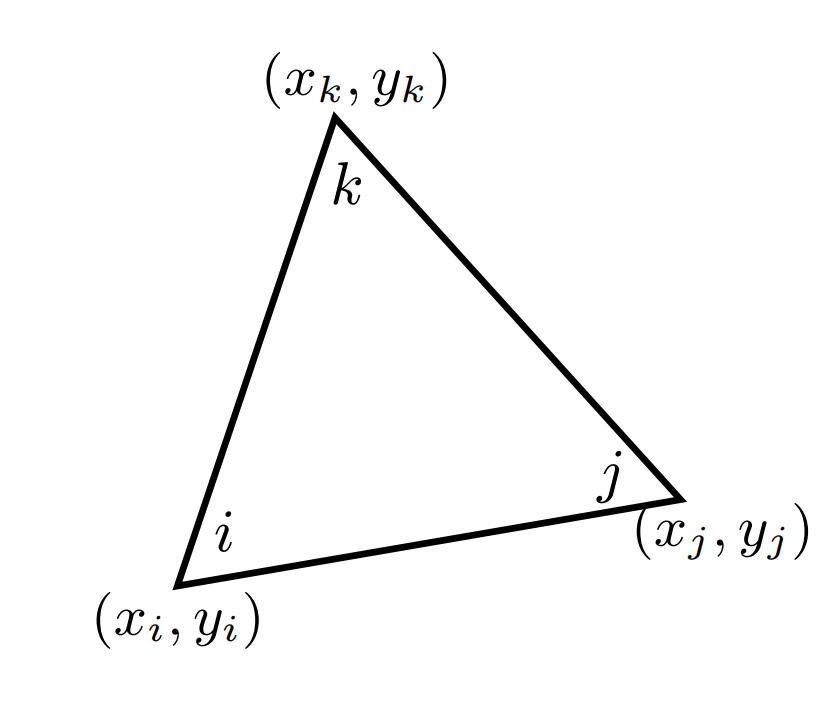
\includegraphics[scale=0.5]{../results/triangle.png}}
\caption{Треугольный элемент}
\label{fig:triangle}
\end{figure}

Обозначим площадь данного треугольника обозначим как A. По формуле, определитель матрицы, составленный из координат вершин треугольника, равен двум площадям треугольника $\left[4\right]$. Соответственно, площадь треугольника можно записать как:

\begin{equation*}
2A = 
\begin{bmatrix}
1 & 1 & 3\\
x_1 & x_2 & x_3 \\ 
y_1 & y_2 & y_3
\end{bmatrix}
= (x_2 y_3 - x_3 y_2) + (x_3 y_1 - x_1 y_3) + (x_1 y_2 - x_2 y_1)
\end{equation*}

\newpage

Для получения функции перемещений для элемента запишем в общем случае функцию $u(x, y)$, зависящую от переменных $x, y$ и интерполируем её линейной функцией $\left[4\right]$:

\begin{equation}\label{main_formula}
u(x, y) = \alpha_1 + \alpha_2 x + \alpha_3 y,
\end{equation} 

где $a_1, a_2, a_3$ - произвольные коэффициенты. Теперь введём аппроксимацию данной функции для треугольного элемента. Обозначим значения функции перемещений в узлах конечного элемента как $u(x_1, y_1), u(x_2, y_2), u(x_3, y_3)$. С помощью данных узловых значений мы сможем получить коэффициенты формулы \ref{main_formula}. Запишем её как:
\begin{equation}\label{system}
\left\{\begin{matrix}
u_1 = u(x_1, y_1) = \alpha_1 + \alpha_2 x_1 + \alpha_3 y_1\\
u_2 = u(x_2, y_2) = \alpha_1 + \alpha_2 x_2 + \alpha_3 y_2 \\
u_3 = u(x_3, y_3) = \alpha_1 + \alpha_2 x_3 + \alpha_3 y_3 
\end{matrix}\right.
\end{equation}

Разрешим систему \ref{system} относительно $\alpha_i$ и подставим получившиеся коэффициенты в \ref{main_formula}, получим, что

\begin{equation*}
u = N_i u_i + N_j u_j + N_k u_k,
\end{equation*}
где $N_m = \frac{1}{2A}(a_m + b_m x + c_m y)$ - функция формы, равная единице в узле $(x_m, y_m)$ и нулю в прочих двух узлах. Коэффициенты $a_m, b_m, c_m$, полученные в уравнении функции формы, вычисляются как

\begin{equation*}
\left\{\begin{matrix}
a_i = x_j y_k - x_k y_j \\
b_i = y_j - y_k \\
c_i = x_k - x_j
\end{matrix}\right.
\
\left\{\begin{matrix}
a_j = x_k y_i - x_i y_k \\
b_j = y_k - y_i \\
c_j = x_i - x_k
\end{matrix}\right.
\
\left\{\begin{matrix}
a_k = x_i y_j - x_j y_i \\
b_k = y_i - y_j \\
c_k = x_j - x_i
\end{matrix}\right.
\end{equation*}

В качестве функций формы для треугольного элемента возьмём бариоцентрические координаты или $L$ - координаты: $N_i = L_1, N_j = L_2, N_k = L_3$ $\left[5\right]$. 

\newpage

\begin{figure}[h]
\center{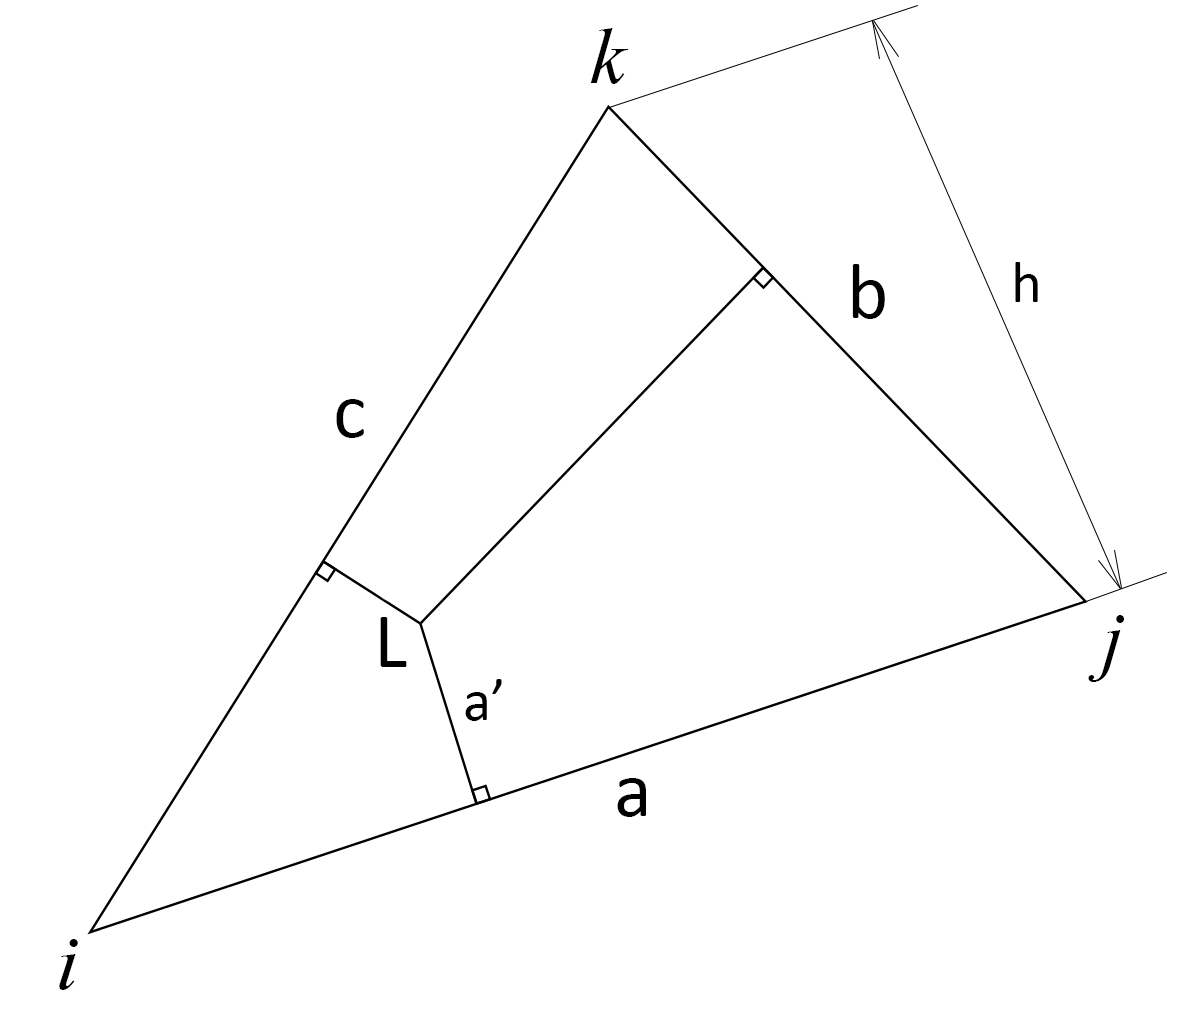
\includegraphics[scale=0.3]{../results/L.png}}
\caption{Бариоцентрические координаты}
\label{fig:bario}
\end{figure}

L-координата представляет собой отношение расстояния из выбранной точки до любой из сторон треугольника к высоте, опущенной из противолежащей вершины на выбранную сторону треугольника. Величина $L_i$ меняется от нуля до единицы, причём в узле i с координатами $(x_i, y_i)$ L-координата равна единице, в то время как в прочих вершинах треугольника бариоцентрическая координата равна нулю.

Координаты случайной точки в декартовой системе координат можно выразить через бариоцентрические координаты:

\begin{eqnarray*}
x = L_1 x_i + L_2 x_j + L_3 x_k \\
y = L_1 y_i + L_2 y_j + L_3 y_k
\end{eqnarray*}

Выгода использования бариоцентрических координат заключается в упрощении вычисления интегралов по площади треугольного элемента или вдоль сторон треугольного элемента:

\begin{equation}
\int_l {(L_1)^a (L_2)^b dl} = \frac{a! b!}{(a + b + 1)!} l
\end{equation}

\begin{equation}
\int_S {(L_1)^a (L_2)^b (L_3)^c dS} = \frac{a! b! c!}{(a + b + c + 2)!}2S
\end{equation}

\newpage

\subsection{Численное решение задачи деформирования упругих тел}

Запишем локальную матрицу жёсткости треугольного элемента:

\begin{equation}\label{main}
K_l = \int_V {\mathbf{B}_l^T \; \mathbf{D} \; \mathbf{B}_l dx dy},
\end{equation}

где матрицы $\mathbf{B}$ и $\mathbf{D}$ получены из векторов тензора напряжений

\begin{equation}
\bm{\sigma} = \mathbf{D} \bm{\varepsilon},
\end{equation}
где
\begin{equation}
\mathbf{D} = 
\begin{pmatrix}
\lambda + 2\mu & \lambda & 0 \\ 
\lambda & \lambda + 2\mu & 0 \\ 
0 & 0 & 2\mu 
\end{pmatrix}
\end{equation}

\begin{equation}
\bm{\varepsilon} =
\begin{pmatrix}
\varepsilon_{xx}\\ 
\varepsilon_{yy}\\ 
\varepsilon_{xy}
\end{pmatrix}
\end{equation}

 и тензора деформаций

\begin{equation}
\bm{\sigma} = \mathbf{B} \bm{u},
\end{equation}
где
\begin{equation}
\mathbf{B} = 
\begin{pmatrix}
\frac{\partial}{\partial x} & 0 \\
0 & \frac{\partial}{\partial y} \\
\frac{1}{2}\frac{\partial}{\partial y} & \frac{1}{2}\frac{\partial}{\partial x}
\end{pmatrix}
\begin{pmatrix}
N_1 & 0 & N_2 & 0 & N_3 & 0 \\
0 & N_1 & 0 & N_2 & 0 & N_3
\end{pmatrix}
\end{equation}


Домножим в уравнении \ref{main} вектор $B_l^T$ на матрицу $\mathbf{D}$, проведём преобразования и получим итоговое уравнение $\left[8\right]$:
\begin{equation}
K_l = \frac{1}{4A}
\begin{bmatrix}
b_i & 0 & \frac{c_i}{2}\\ 
0 & c_i & \frac{b_i}{2}
\end{bmatrix}
\begin{bmatrix}
\lambda + 2\mu & \lambda & 0 \\ 
\lambda & \lambda + 2\mu & 0 \\ 
0 & 0 & 2\mu 
\end{bmatrix}
\begin{bmatrix}
b_j & 0 \\
0 & c_j \\
\frac{c_j}{2} & \frac{b_j}{2}
\end{bmatrix}
\end{equation}

\newpage

После перемножения матриц получим итоговую локальную матрицу жёсткости размера 2x2. По итогу, глобальная система уравнений имеет вид

\begin{equation}
\mathbf{Ku} = \mathbf{R},
\end{equation}
где матрица $\mathbf{K}$ - глобальная матрица жёсткости размера (2n)x(2n), $\mathbf{u} = (u_{x1}, u_{y1}, \ldots, u_{xn}, u_{yn})$, $\mathbf{R}$ - вектор правой части размерности (2n)x1.
\newpage

\section{Краткое описание программы}

Программа предназначена для проведения серии расчётов для численного решения задачи деформирования упругих тел для четырёх тестовых задач. В программе реализованы базовый методо решения задач на всей области без МДО, мультипликативный метод Шварца, аддитивный метод Шварца и двухуровневый аддитивный метод Шварца. Исходным языком программирования для программы является Python. Среда разработки - Visual Studio Code. На рисунке \ref{fig:scheme} продемонстрирован алгоритм программы в виде блок-схемы. 

\begin{figure}[h]
\center{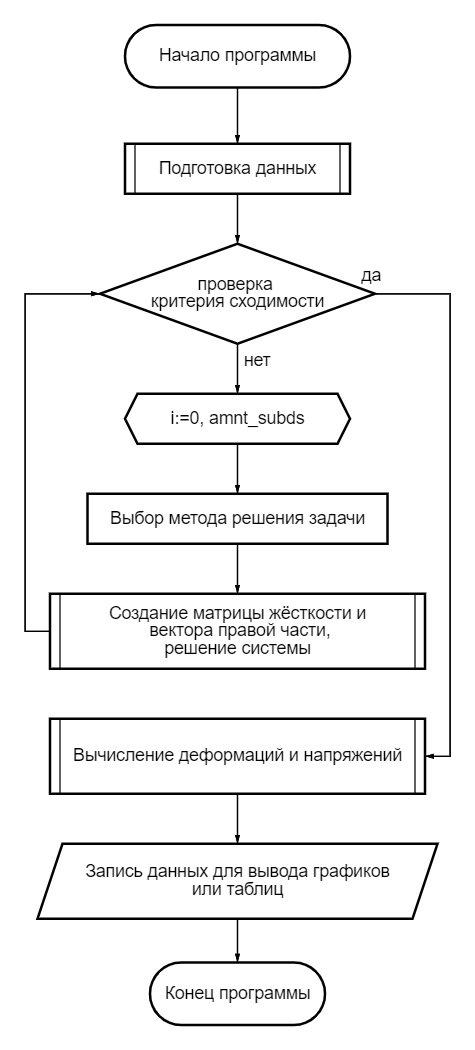
\includegraphics[scale=0.45]{../results/diagram.png}}
\caption{Блок-схема программы}
\label{fig:scheme}
\end{figure}

\newpage

Подготовка данных заключается в вводе геометрических параметров области, кинематических и силовых условий, выборе модели материала, задании свойств материала и задания сетки с выбранным шагом h. Входными данными для программы являются файл {task}.dat, предназначенный для введения параметров задачи и области и файл {h}.msh, созданный автоматизированной импортированной библиотекой "meshio" и содержащий описание выбранной сетки.

Используя программу, можно сохранить полученные результаты в типизированные файлы формата .csv для таблиц данных, либо в файлы формата .png для иллюстраций и графиков.

\newpage

\section{Результаты численных расчётов}

В данном разделе будут приведены расчёты четырёх тестовых задач с использованием четырёх методов. Для каждой из задач для базового случая будут приведены графики распределения напряжений вдоль поверхности, к которой приложено давление, а также графики распределения перемещений на всей расчётной области.

Для методов декомпозиции области расчётные области будут разбиты на заданное количество секторов без перекрытия $\Omega_1, \ldots, \Omega_M$ в зависимости от задачи, где M - число подобластей. Также стоит заметить, что каждая подобласть $\Omega_i$ ($i = 1,\ldots,M$) в зависимости от задачи обладает своими размерными характеристиками. Подобласть $G_i$ соответствует объединению подобласти $\Omega_i$ и дополнительных участков соседних подобластей $\Omega_{i-1}$ и $\Omega_{i+1}$. Размеры этих дополнительных участков зависят от относительного коэффициента перекрытия (отношение размера перекрытия к размеру подобласти $\Omega_i$).

Итерационный процесс для мультипликативного, аддитивного и двухуровневого аддитивного методов продолжается до тех пор, пока не выполнится условие критерия останова $u_{err}$ для перемещений:

\begin{equation*}
u_{err} = \sqrt{\left(\sum_{k = 1}^{N_p} s_k \left(\frac{u_{k}^{m+1} - u_{k}^{m}}{u_{k}^{m+1}} \right)^2\right) / \left(\sum_{k = 1}^{N_{p}} s_k\right)} < \varepsilon_0,
\end{equation*}
где $s_k$ - суммарная площадь элементов сетки, в которые входит $k$-й узел, разделённая на количество узлов в элементе, $N_{elem}$ - количество узлов сетки, $u_{k}^{m+1}$ - решение на текущей итерации, $u_{k}^{m}$ - решение на предыдущей итерации.

Дополнительно для каждой из задач для методов декомпозиции будут приведены таблицы зависимости количества итераций от относительного коэффициента перекрытия.

\newpage

\subsection{Первая тестовая задача}

На рис. \ref{fig:task_\taskNum_scheme} представлена расчётная область - прямоугольник, закреплённый с левой и правой стороны по оси OX и с нижней стороны по оси OY. Сверху действует распределённая нагрузка $p = 50$ МПа. Ширина тела $a = 2$ см, высота тела $b = 1$ см.

\begin{figure}[h]
\center{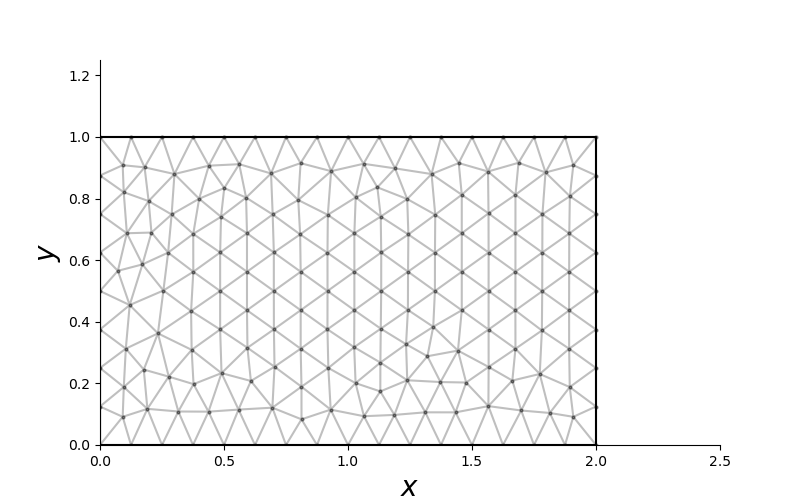
\includegraphics[scale=0.8]{../results/\area/\task/core/area_diagram.png}}
\caption{Схема расчётной области (h = 0.125)}
\label{fig:task_\taskNum_scheme}
\end{figure}

Для решения поставленной задачи примем, что материал тела имеет следующие параметры: модуль Юнга $E = 70$ ГПа, коэффициент Пуассона $\mu = 0.34$. 

Для исследования зависимости сходимости метода от размерности итоговой системы линейных уравнений рассмотрены три расчётные сетки с шагами $h = 0.05$ (количество узлов - 994), $h = 0.025$ (количество узлов - 3812), $h = 0.0125$ (количество узлов - 15006).

Для аддитивного метода Шварца итерационный параметр $\alpha = 0.5$.

\newpage

Для решения задачи методами декомпозиции области расчётная область разбивается по оси OX на заданное количество прямоугольных областей без перекрытия $\Omega_1, \ldots, \Omega_M$. Характерные размеры каждой подобласти: ширина подобласти $a_M = a / M$, высота подобласти совпадает с высотой тела $b_M = b$. На рис. \ref{fig:task_\taskNum_decomposition} представлена расчётная область первой тестовой задачи, разбитая на две подобласти.

\begin{figure}[h]
\center{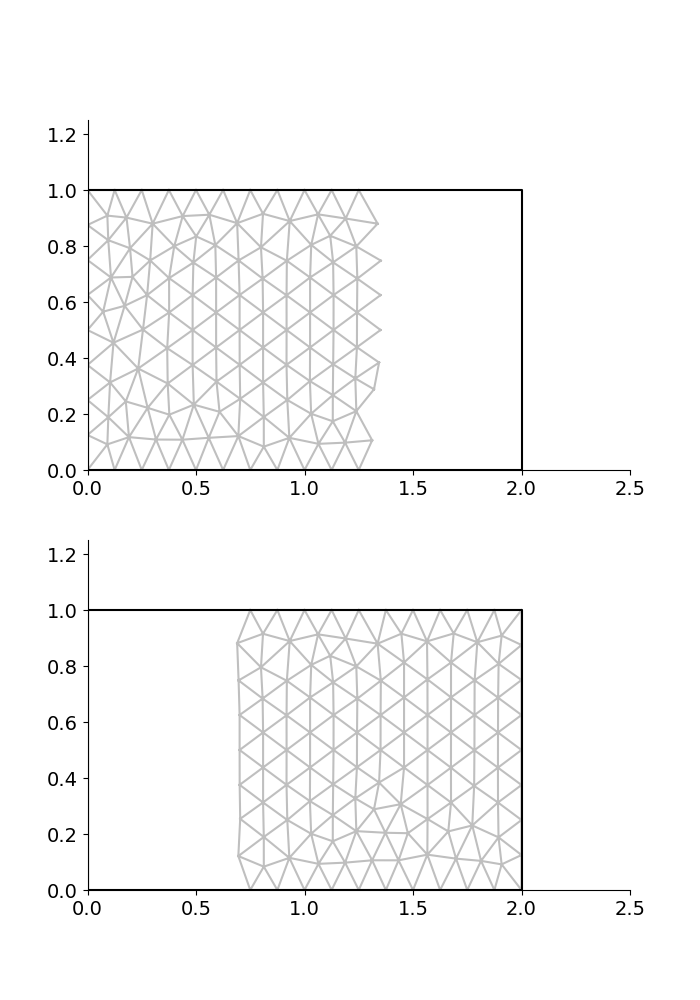
\includegraphics[scale=0.75]{../results/\area/\task/core/area_decomposition.png}}
\caption{Схема декомпозиции расчётной области (M = 2, h = 0.125)}
\label{fig:task_\taskNum_decomposition}
\end{figure}

\newpage

На рис. \ref{fig:task_\taskNum_basic_displacement_distribution} приведено распределение радиальных перемещений, полученных при решении задачи во всей расчётной области базовым методом, на рис. \ref{fig:task_\taskNum_basic_pressure_distribution_y} - распределение погрешностей узловых напряжений $\Delta\sigma_y$, полученных при решении задачи во всей расчётной области, причём полная погрешность вычисляется по формуле $\sigma_y = \tilde{\sigma_y} + \Delta \sigma_y$, где $\tilde{\sigma_y}$ = 50 МПа.

\begin{figure}[h]
\center{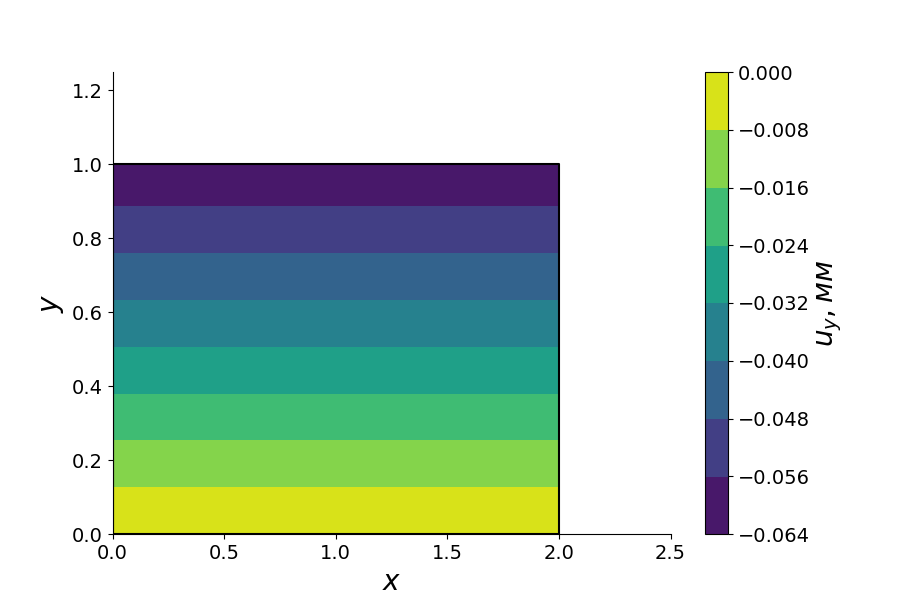
\includegraphics[scale=0.55]{../results/\area/\task/core/displacement_distribution.png}}
\caption{Распределение перемещений во всей расчётной области (h = 0.125)}
\label{fig:task_\taskNum_basic_displacement_distribution}
\center{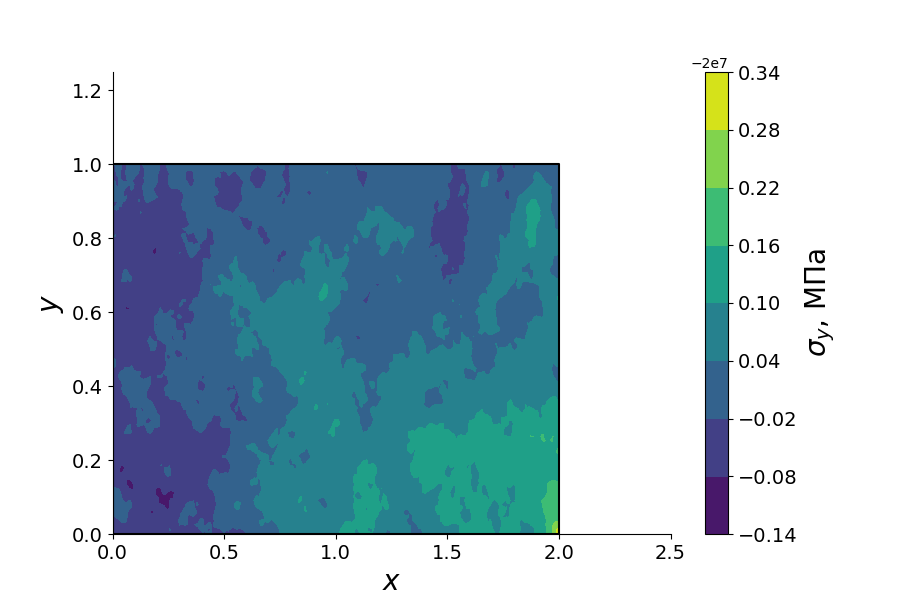
\includegraphics[scale=0.55]{../results/\area/\task/core/pressure_distribution_y.png}}
\caption{Распределение узловых напряжений во всей расчётной области (h = 0.125)}
\label{fig:task_\taskNum_basic_pressure_distribution_y}
\end{figure}

\newpage

\subsubsection{Мультипликативный метод Шварца}

В таблице \ref{table:task_\taskNum_mult_iters} представлено количество итераций в зависимости от количества подобластей и шага сетки при использовании мультипликативного метода Шварца (коэффициент захлёста для подобластей равен 0.3). Анализ полученных результатов показал, что:
\begin{itemize}
\item количество итераций не зависит от шага сетки;
\item при увеличении числа подобластей количество итераций увеличивается (при увеличении количества подобластей количество итераций увеличивается примерно в $M^2$ раз);
\end{itemize}

\begin{table}[h]
\caption{Количество итераций в зависимости от количества подобластей и шага сетки}
\csvloop{
	file = ../results/\area/\task/schwarz_multiplicative/iters.csv,
	head to column names,
	before reading = \centering\sisetup{table-number-alignment=center},
	tabular = {
		@{} |
		p{3cm} |
		c | 
		c |
		c |
		c |
		@{}
	},
	table head = \hline Количество подобластей (M) & \text{h = 0.05} & \text{h = 0.025} & \text{h = 0.0125} & \text{h = 0.00625} \\\hline,
	command = \amnt & \0 & \1 & \2 & \3,
	late after line = \\\hline
}
\label{table:task_\taskNum_mult_iters}
\end{table}

\newpage

\subsubsection{Аддитивный метод Шварца}

В таблице \ref{table:task_\taskNum_add_iters} представлено количество итераций в зависимости от количества подобластей и шага сетки при использовании аддитивного метода Шварца (коэффициент захлёста для подобластей равен 0.3). Анализ полученных результатов показал, что:
\begin{itemize}
\item количество итераций несильно зависит от шага сетки;
\item при увеличении числа подобластей количество итераций увеличивается (при увеличении количества подобластей количество итераций увеличивается примерно в $M^2$ раз);
\item количество итераций по сравнению со случаем применения мультипликативного метода Шварца выросло почти в 4 раза;
\end{itemize}

\begin{table}[h]
\caption{Количество итераций в зависимости от количества подобластей и шага сетки}
\csvloop{
	file = ../results/\area/\task/schwarz_additive/iters.csv,
	head to column names,
	before reading = \centering\sisetup{table-number-alignment=center},
	tabular = {
		@{} |
		p{3cm} |
		c | 
		c |
		c |
		c |
		@{}
	},
	table head = \hline Количество подобластей (M) & \text{h = 0.05} & \text{h = 0.025} & \text{h = 0.0125} & \text{h = 0.00625} \\\hline,
	command = \amnt & \0 & \1 & \2 & \3,
	late after line = \\\hline
}
\label{table:task_\taskNum_add_iters}
\end{table}

\newpage

\subsubsection{Двухуровневый аддитивный метод Шварца}
Для двухуровневого аддитивного метода кроме основной сетки в расчётной области зададим грубую сетку, удовлетворяющую условиям включения всех узлов мелкой сетки в элементы грубой сетки и соответствия размеров областей. 

В таблице \ref{table:task_\taskNum_add2_coarse} представлено количество итераций в зависимости от количества подобластей и шага грубой сетки при использовании двухуровневого аддитивного метода Шварца для шага мелкой сетки h = 0.0125 (коэффициент захлёста для подобластей равен 0.3).

Анализ данной таблицы показывает, что для расчётов рациональнее взять шаг H = 0.125, так как в этом случае количество итераций незначительно зависит от количества подобластей.

На рис. \ref{fig:task_01_area_coarse} изображена расчётная схема области с грубой сеткой при H = 1.

\begin{figure}[h]
\center{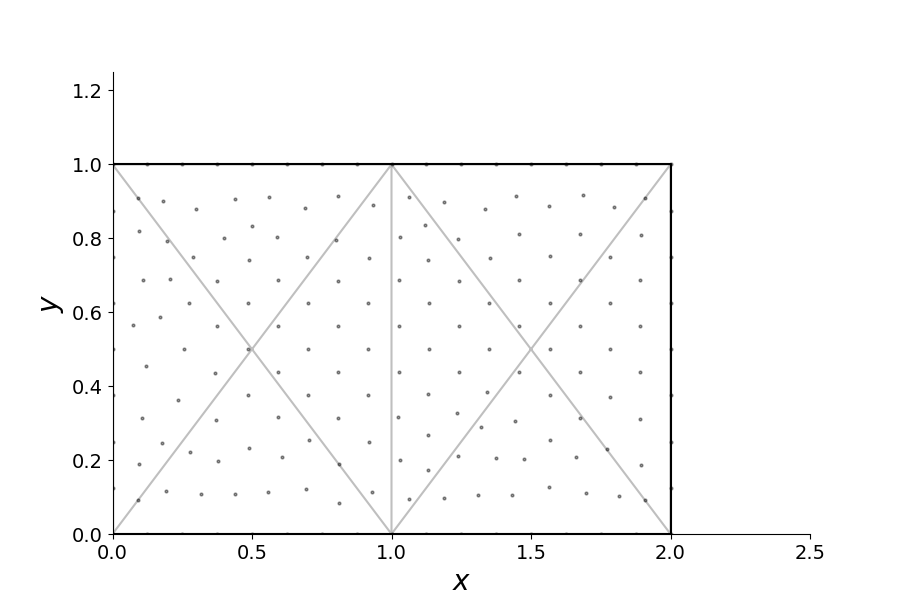
\includegraphics[scale=0.7]{../results/\area/\task/core/area_coarse_rectangle.png}}
\caption{Схема расчётной области с прямоугольной областью в качестве грубой области \\ (h = 0.125, H = 1)}
\label{fig:task_\taskNum_area_coarse}
\end{figure}

\newpage

\begin{table}[h]
\caption{Количество итераций в зависимости от количества подобластей и шага грубой сетки для двухуровневого аддитивного метода Шварца (h = 0.0125)}
\csvloop{
	file = ../results/\area/\task/schwarz_two_level_additive/iters_rectangle.csv,
	head to column names,
	before reading = \centering\sisetup{table-number-alignment=center},
	tabular = {
		@{} |
		c |
		c | 
		c |
		c |
		c |
		@{}
	},
	table head = \hline Количество подобластей & \text{H = 1} & \text{H = 0.5} & \text{H = 0.025} & \text{H = 0.125} \\\hline,
	command = \amnt & \0 & \1 & \2 & \3,
	late after line = \\\hline
}
\label{table:task_\taskNum_add2_coarse}
\end{table}

В таблице \ref{table:task_\taskNum_add2_iters} представлено количество итераций в зависимости от количества подобластей и шага сетки при использовании двухуровневого аддитивного метода Шварца для первой тестовой задачи при H = 0.125 (коэффициент захлёста для подобластей равен 0.3). Анализ полученных результатов показал, что:
\begin{itemize}
\item количество итераций не зависит от шага сетки;
\item при увеличении числа подобластей количество итераций не меняется;
\end{itemize}

\begin{table}[h]
\caption{Количество итераций в зависимости от количества подобластей и шага сетки для двухуровневого аддитивного метода Шварца (H = 0.125)}
\csvloop{
	file = ../results/\area/\task/schwarz_two_level_additive/iters.csv,
	head to column names,
	before reading = \centering\sisetup{table-number-alignment=center},
	tabular = {
		@{} |
		c |
		c | 
		c |
		c |
		c |
		@{}
	},
	table head = \hline Количество подобластей & \text{h = 0.05} & \text{h = 0.025} & \text{h = 0.0125} & \text{h = 0.00625} \\\hline,
	command = \amnt & \0 & \1 & \2 & \3,
	late after line = \\\hline
}
\label{table:task_\taskNum_add2_iters}
\end{table}

В таблице \ref{table:task_\taskNum_iters_overlap} рассмотрена зависимость количества итераций от различных вариантов МДО и коэффициента относительного захлёста при M = 4, h = 0.025 и H = 0.125. 

Из таблицы видно, что при росте коэффициента относительного захлёста количество итераций уменьшается.

\begin{table}[h]
\caption{Количество итераций в зависимости от метода декомпозиции области и коэффициента относительного захлёста (M = 4, h = 0.025, H = 0.125)}
\csvloop{
	file = ../results/\area/\task/core/iters_overlap.csv,
	head to column names,
	before reading = \centering\sisetup{table-number-alignment=center},
	tabular = {
		@{} |
		c |
		c |
		c |
		c |
		@{}
	},
	table head = \hline Коэффициент относительного захлёста & 0.2 & 0.3 & 0.4 \\\hline,
	command = \method & \0 & \1 & \2,
	late after line = \\\hline
}
\label{table:task_\taskNum_iters_overlap}
\end{table}

\newpage
В таблице \ref{table:task_\taskNum_iters_cg} приведены количество итераций, за которое сходится метод сопряженных градиентов, при решении задачи во всей области без методов декомпозиции, а также общее количество итераций, за которое сходится метода сопряженных градиентов для каждой локальной задачи, при решении задачи во всей области двухуровневым аддитивным методом Шварца.

В таблице \ref{table:task_\taskNum_iters_cg_rel} приведены отношения размерностей систем, отношения количества итераций при решении задачи во всей области без методов декомпозиции, отношения количества итераций в соответствии с теорией и отношения количества итераций при решении задачи во всей области двухуровневым аддитивным методом Шварца.

Из таблицы \ref{table:task_\taskNum_iters_cg_rel} видно, что отношения для базового метода и двухуровневого метода практически идентичны благодаря тому, что общее количество итераций для двухуровневого аддитивного метода Шварца не меняется при изменении размерности системы. На рис. \ref{fig:task_01_iters_cg} наглядно продемонстрированы результаты, полученные в таблице \ref{table:task_\taskNum_iters_cg_rel}.

\begin{table}[h]
\caption{Количество итераций метода сопряженных градиентов в зависимости от размера СЛАУ и метода решения задачи}
\csvloop{
	file = ../results/\area/\task/core/iters_cg.csv,
	head to column names,
	before reading = \centering\sisetup{table-number-alignment=center},
	tabular = {
		@{} |
		c |
		c |
		c |
		@{}
	},
	table head = \hline Размерность системы & Базовый метод & Двухуровневый аддитивный МДО \\\hline,
	command = \index & \basic & \8,
	late after line = \\\hline
}
\label{table:task_\taskNum_iters_cg}
\end{table}

\begin{table}[h]
\caption{Отношение количества итераций метода сопряженных градиентов}
\csvloop{
	file = ../results/\area/\task/core/iters_cg_rel.csv,
	head to column names,
	before reading = \centering\sisetup{table-number-alignment=center},
	tabular = {
		@{} |
		p{3.0cm} |
		p{3.0cm} |
		l |
		l |
		p{4.0cm} |
		@{}
	},
	table head = \hline Размерность системы & Отношение размеров & Теория & Базовый метод & Двухуровневый аддитивный МДО \\\hline,
	command = \index & \N & \theory & \basic & \8,
	late after line = \\\hline
}
\label{table:task_\taskNum_iters_cg_rel}
\end{table}

\newpage

В таблице \ref{table:task_\taskNum_time_cg} приведены временные затраты, необходимые для решения задачи во всей области без методов декомпозиции, а также временные затраты для решения задачи во всей области двухуровневым аддитивным методом Шварца.

В таблице \ref{table:task_\taskNum_time_cg_rel} приведены отношения размерностей систем, отношения временных затрат при решении задачи во всей области без методов декомпозиции, отношения временных затрат в соответствии с теорией и отношения временных затрат при решении задачи во всей области двухуровневым аддитивным методом Шварца.

Из таблицы \ref{table:task_\taskNum_time_cg_rel} видно, что отношение временных затрат для двухуровневого аддитивного метода Шварца лучше, чем для теоретического случая и тем более для базового метода решения задачи без применения МДО. На рис. \ref{fig:task_\taskNum_time_cg} наглядно продемонстрированы результаты, полученные в таблице \ref{table:task_\taskNum_time_cg_rel}.

\begin{table}[h]
\caption{Время, затраченное на метод сопряженных градиентов, в зависимости от размера СЛАУ и метода решения задачи}
\csvloop{
	file = ../results/\area/\task/core/time_cg.csv,
	head to column names,
	before reading = \centering\sisetup{table-number-alignment=center},
	tabular = {
		@{} |
		c |
		c |
		c |
		@{}
	},
	table head = \hline Размер СЛАУ & Базовый метод & Двухуровневый аддитивный МДО \\\hline,
	command = \index & \basic & \8,
	late after line = \\\hline
}
\label{table:task_\taskNum_time_cg}
\end{table}

\begin{table}[h]
\caption{Отношение затраченного времени на метод сопряженных градиентов}
\csvloop{
	file = ../results/\area/\task/core/time_cg_rel.csv,
	head to column names,
	before reading = \centering\sisetup{table-number-alignment=center},
	tabular = {
		@{} |
		p{3.0cm} |
		p{3.0cm} |
		l |
		l |
		p{4.0cm} |
		@{}
	},
	table head = \hline Размер СЛАУ & Теория & Базовый метод & Двухуровневый аддитивный МДО \\\hline,
	command = \index & \theory & \basic & \8,
	late after line = \\\hline
}
\label{table:task_\taskNum_time_cg_rel}
\end{table}

\newpage

\begin{figure}[H]
\center{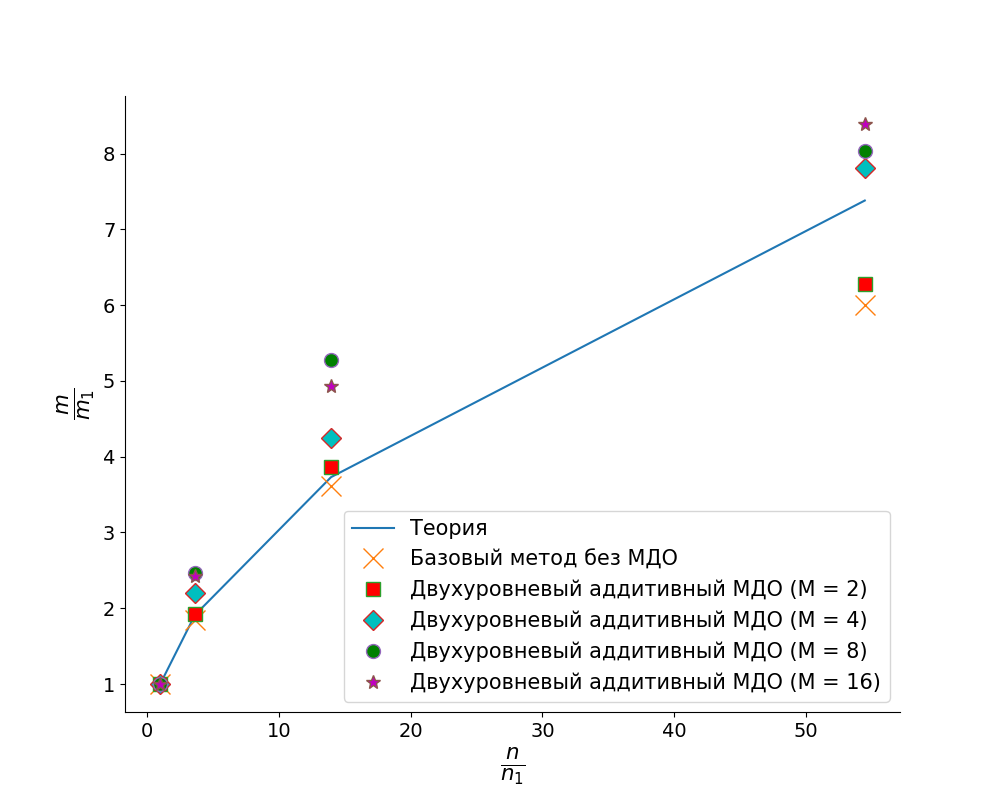
\includegraphics[scale=0.5]{../results/\area/\task/core/iters_cg.png}}
\caption{График отношений количества итераций}
\label{fig:task_\taskNum_iters_cg}
\end{figure}
\begin{figure}[H]
\center{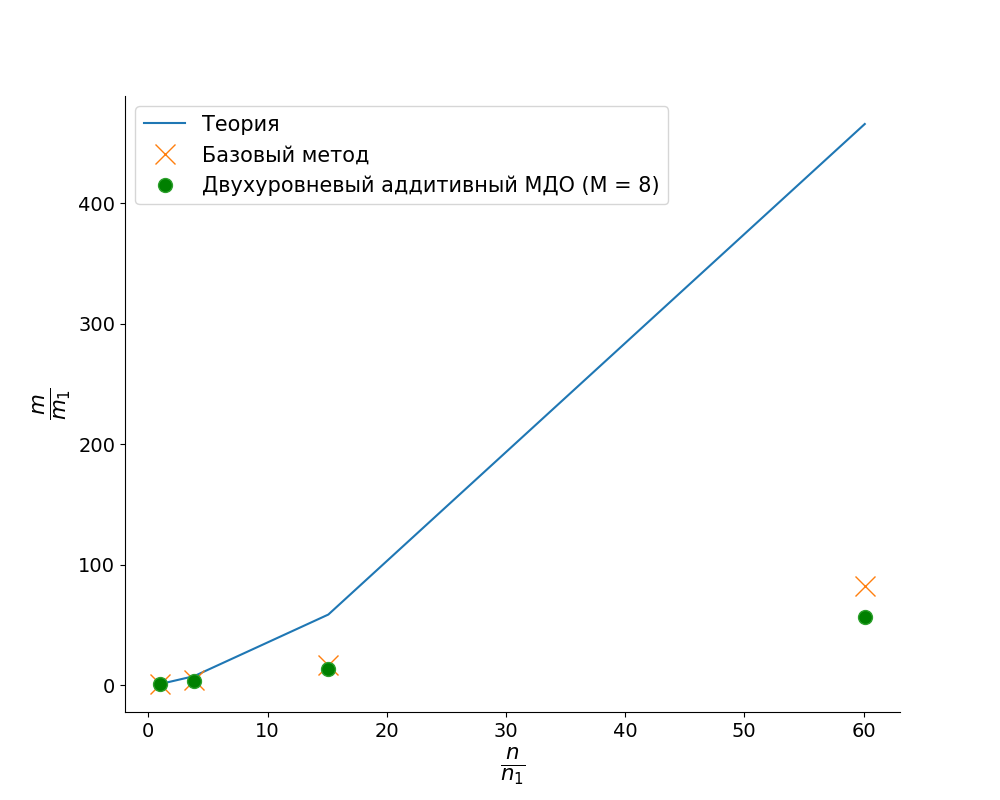
\includegraphics[scale=0.5]{../results/\area/\task/core/time_cg.png}}
\caption{График отношений временных затрат}
\label{fig:task_\taskNum_time_cg}
\end{figure}

\newpage

\subsection{Вторая тестовая задача}

\renewcommand{\task}{2_fixes}
\renewcommand{\taskNum}{02}

На рис. \ref{fig:task_\taskNum_scheme} представлена расчётная область - прямоугольник, закреплённый с левой стороны по оси OX и с нижней стороны по оси OY. Сверху действует распределённая нагрузка $p = 50$ МПа. Ширина тела $a = 2$ см, высота тела $b = 1$ см.

\begin{figure}[h]
\center{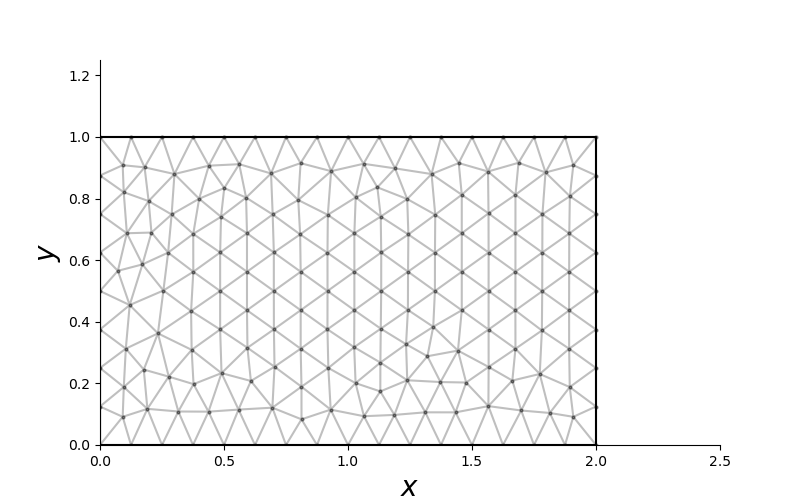
\includegraphics[scale=0.9]{../results/\area/\task/core/area_diagram.png}}
\caption{Схема расчётной области (h = 0.125)}
\label{fig:task_\taskNum_scheme}
\end{figure}

Для решения поставленной задачи примем, что материал тела имеет следующие параметры: модуль Юнга $E = 70$ ГПа, коэффициент Пуассона $\mu = 0.34$. 

Для исследования зависимости сходимости метода от размерности итоговой системы линейных уравнений рассмотрены три расчётные сетки с шагами $h = 0.05$ (количество узлов - 994), $h = 0.025$ (количество узлов - 3812), $h = 0.0125$ (количество узлов - 15006).

Для аддитивного метода Шварца итерационный параметр $\alpha = 0.5$.

\newpage

Для решения задачи методами декомпозиции области расчётная область разбивается по оси OX на заданное количество прямоугольных областей без перекрытия $\Omega_1, \ldots, \Omega_M$. Характерные размеры каждой подобласти: ширина подобласти $a_M = a / M$, высота подобласти совпадает с высотой тела $b_M = b$. На рис. \ref{fig:task_\taskNum_decomposition} представлена расчётная область первой тестовой задачи, разбитая на две подобласти.

\begin{figure}[h]
\center{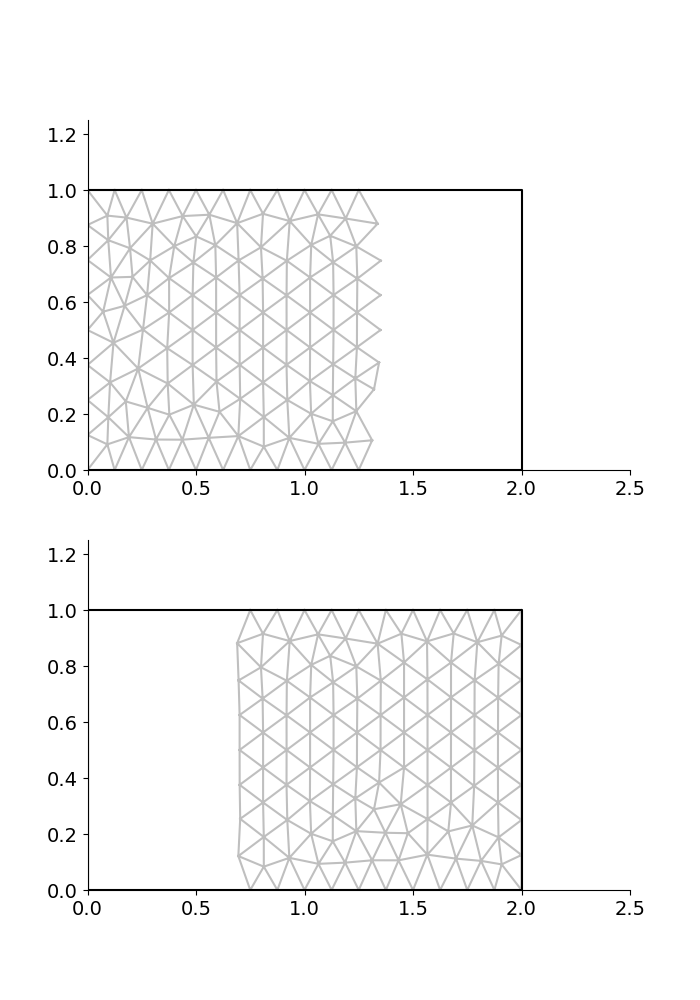
\includegraphics[scale=0.75]{../results/\area/\task/core/area_decomposition.png}}
\caption{Схема декомпозиции расчётной области (M = 2, h = 0.125)}
\label{fig:task_\taskNum_decomposition}
\end{figure}

\newpage

На рис. \ref{fig:task_\taskNum_basic_displacement_distribution} приведено распределение радиальных перемещений, полученных при решении задачи во всей расчётной области базовым методом, на рис. \ref{fig:task_\taskNum_basic_pressure_distribution_y} - распределение погрешностей узловых напряжений $\Delta\sigma_y$, полученных при решении задачи во всей расчётной области, причём полная погрешность вычисляется по формуле $\sigma_y = \tilde{\sigma_y} + \Delta \sigma_y$, где $\tilde{\sigma_y}$ = 50 МПа.

\begin{figure}[h]
\center{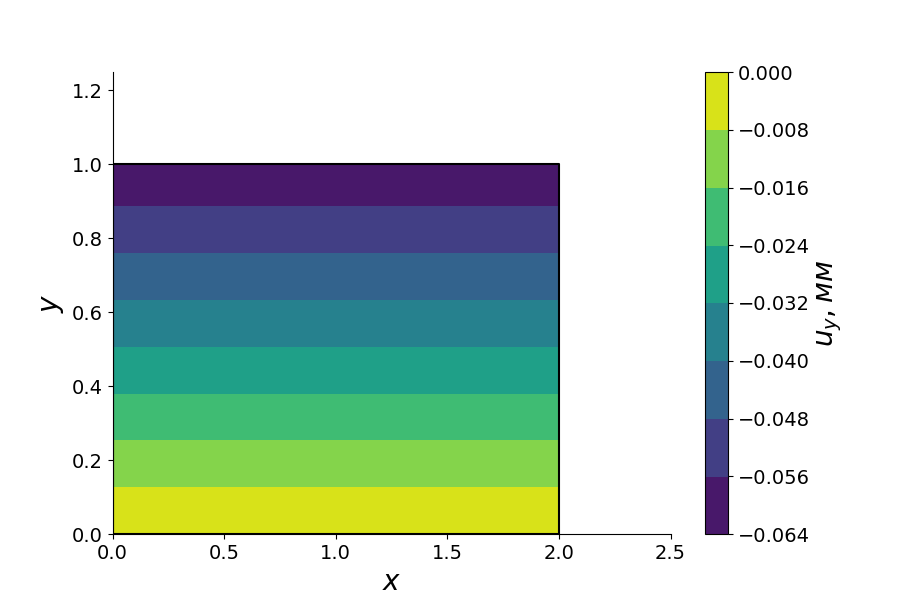
\includegraphics[scale=0.55]{../results/\area/\task/core/displacement_distribution.png}}
\caption{Распределение перемещений во всей расчётной области (h = 0.125)}
\label{fig:task_\taskNum_basic_displacement_distribution}
\center{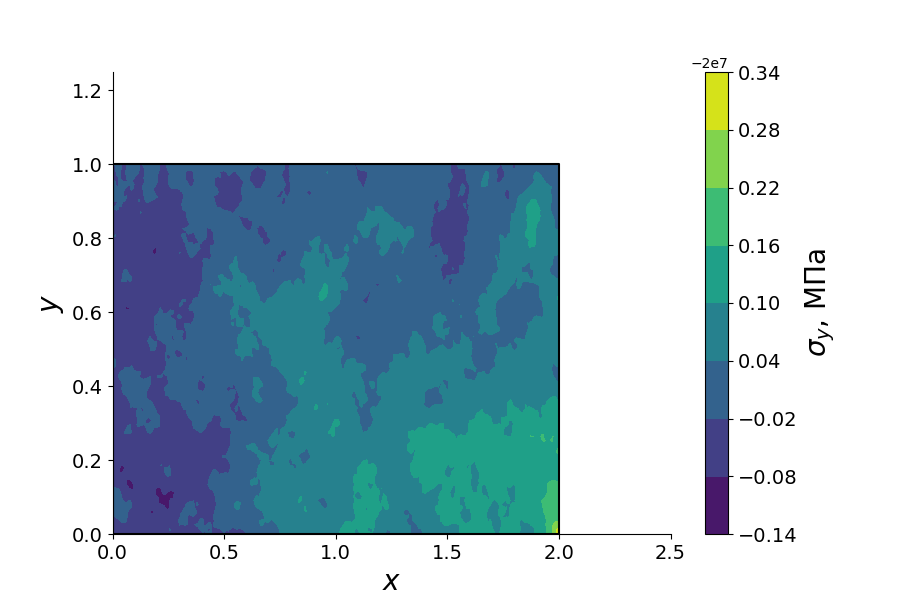
\includegraphics[scale=0.55]{../results/\area/\task/core/pressure_distribution_y.png}}
\caption{Распределение узловых напряжений во всей расчётной области (h = 0.125)}
\label{fig:task_\taskNum_basic_pressure_distribution_y}
\end{figure}

\newpage

\subsubsection{Мультипликативный метод Шварца}

В таблице \ref{table:task_\taskNum_mult_iters} представлено количество итераций в зависимости от количества подобластей и шага сетки при использовании мультипликативного метода Шварца (коэффициент захлёста для подобластей равен 0.3). Анализ полученных результатов показал, что:
\begin{itemize}
\item количество итераций не зависит от шага сетки;
\item при увеличении числа подобластей количество итераций увеличивается (при увеличении количества подобластей количество итераций увеличивается примерно в $M^2$ раз);
\end{itemize}

\begin{table}[h]
\caption{Количество итераций в зависимости от количества подобластей и шага сетки}
\csvloop{
	file = ../results/\area/\task/schwarz_multiplicative/iters.csv,
	head to column names,
	before reading = \centering\sisetup{table-number-alignment=center},
	tabular = {
		@{} |
		p{3cm} |
		c | 
		c |
		c |
		c |
		@{}
	},
	table head = \hline Количество подобластей (M) & \text{h = 0.05} & \text{h = 0.025} & \text{h = 0.0125} & \text{h = 0.00625} \\\hline,
	command = \amnt & \0 & \1 & \2 & \3,
	late after line = \\\hline
}
\label{table:task_\taskNum_mult_iters}
\end{table}

\newpage

\subsubsection{Аддитивный метод Шварца}

В таблице \ref{table:task_\taskNum_add_iters} представлено количество итераций в зависимости от количества подобластей и шага сетки при использовании аддитивного метода Шварца (коэффициент захлёста для подобластей равен 0.3). Анализ полученных результатов показал, что:
\begin{itemize}
\item количество итераций несильно зависит от шага сетки;
\item при увеличении числа подобластей количество итераций увеличивается (при увеличении количества подобластей количество итераций увеличивается примерно в $M^2$ раз);
\item количество итераций по сравнению со случаем применения мультипликативного метода Шварца выросло почти в 4 раза;
\end{itemize}

\begin{table}[h]
\caption{Количество итераций в зависимости от количества подобластей и шага сетки}
\csvloop{
	file = ../results/\area/\task/schwarz_additive/iters.csv,
	head to column names,
	before reading = \centering\sisetup{table-number-alignment=center},
	tabular = {
		@{} |
		p{3cm} |
		c | 
		c |
		c |
		c |
		@{}
	},
	table head = \hline Количество подобластей (M) & \text{h = 0.05} & \text{h = 0.025} & \text{h = 0.0125} & \text{h = 0.00625} \\\hline,
	command = \amnt & \0 & \1 & \2 & \3,
	late after line = \\\hline
}
\label{table:task_\taskNum_add_iters}
\end{table}

\newpage

\subsubsection{Двухуровневый аддитивный метод Шварца}
Для двухуровневого аддитивного метода кроме основной сетки в расчётной области зададим грубую сетку, удовлетворяющую условиям включения всех узлов мелкой сетки в элементы грубой сетки и соответствия размеров областей. 

В таблице \ref{table:task_\taskNum_add2_coarse} представлено количество итераций в зависимости от количества подобластей и шага грубой сетки при использовании двухуровневого аддитивного метода Шварца для шага мелкой сетки h = 0.0125 (коэффициент захлёста для подобластей равен 0.3).

Анализ данной таблицы показывает, что для расчётов рациональнее взять шаг H = 0.125, так как в этом случае количество итераций незначительно зависит от количества подобластей.

На рис. \ref{fig:task_01_area_coarse} изображена расчётная схема области с грубой сеткой при H = 1.

\begin{figure}[h]
\center{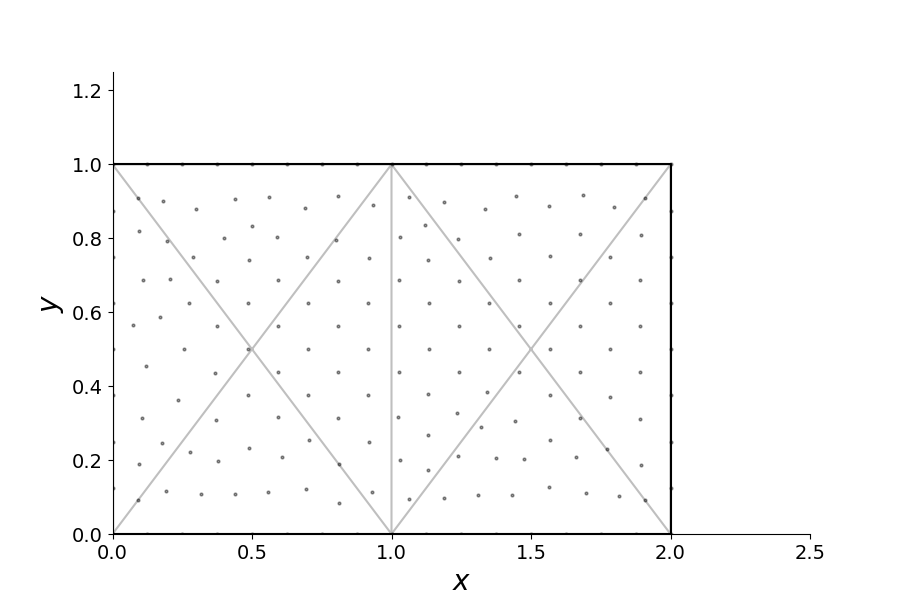
\includegraphics[scale=0.7]{../results/\area/\task/core/area_coarse_rectangle.png}}
\caption{Схема расчётной области с прямоугольной областью в качестве грубой области (h = 0.125, H = 1)}
\label{fig:task_\taskNum_area_coarse}
\end{figure}

\newpage

\begin{table}[h]
\caption{Количество итераций в зависимости от количества подобластей и шага грубой сетки для двухуровневого аддитивного метода Шварца (h = 0.0125)}
\csvloop{
	file = ../results/\area/\task/schwarz_two_level_additive/iters_rectangle.csv,
	head to column names,
	before reading = \centering\sisetup{table-number-alignment=center},
	tabular = {
		@{} |
		c |
		c | 
		c |
		c |
		c |
		@{}
	},
	table head = \hline Количество подобластей & \text{H = 1} & \text{H = 0.5} & \text{H = 0.025} & \text{H = 0.125} \\\hline,
	command = \amnt & \0 & \1 & \2 & \3,
	late after line = \\\hline
}
\label{table:task_\taskNum_add2_coarse}
\end{table}

В таблице \ref{table:task_\taskNum_add2_iters} представлено количество итераций в зависимости от количества подобластей и шага сетки при использовании двухуровневого аддитивного метода Шварца для первой тестовой задачи при H = 0.125 (коэффициент захлёста для подобластей равен 0.3). Анализ полученных результатов показал, что:
\begin{itemize}
\item количество итераций не зависит от шага сетки;
\item при увеличении числа подобластей количество итераций не меняется;
\end{itemize}

\begin{table}[h]
\caption{Количество итераций в зависимости от количества подобластей и шага сетки для двухуровневого аддитивного метода Шварца (H = 0.125)}
\csvloop{
	file = ../results/\area/\task/schwarz_two_level_additive/iters.csv,
	head to column names,
	before reading = \centering\sisetup{table-number-alignment=center},
	tabular = {
		@{} |
		c |
		c | 
		c |
		c |
		c |
		@{}
	},
	table head = \hline Количество подобластей & \text{h = 0.05} & \text{h = 0.025} & \text{h = 0.0125} & \text{h = 0.00625} \\\hline,
	command = \amnt & \0 & \1 & \2 & \3,
	late after line = \\\hline
}
\label{table:task_\taskNum_add2_iters}
\end{table}

В таблице \ref{table:task_\taskNum_iters_overlap} рассмотрена зависимость количества итераций от различных вариантов МДО и коэффициента относительного захлёста при M = 4, h = 0.025 и H = 0.125. Из таблицы видно, что при росте коэффициента относительного захлёста количество итераций уменьшается.

\begin{table}[h]
\caption{Количество итераций в зависимости от метода декомпозиции области и коэффициента относительного захлёста (M = 4, h = 0.025, H = 0.125)}
\csvloop{
	file = ../results/\area/\task/core/iters_overlap.csv,
	head to column names,
	before reading = \centering\sisetup{table-number-alignment=center},
	tabular = {
		@{} |
		c |
		c |
		c |
		c |
		@{}
	},
	table head = \hline Коэффициент относительного захлёста & 0.2 & 0.3 & 0.4 \\\hline,
	command = \method & \0 & \1 & \2,
	late after line = \\\hline
}
\label{table:task_\taskNum_iters_overlap}
\end{table}

\newpage
В таблице \ref{table:task_\taskNum_iters_cg} приведены количество итераций, за которое сходится метод сопряженных градиентов, при решении задачи во всей области без методов декомпозиции, а также общее количество итераций, за которое сходится метода сопряженных градиентов для каждой локальной задачи, при решении задачи во всей области двухуровневым аддитивным методом Шварца.

В таблице \ref{table:task_\taskNum_iters_cg_rel} приведены отношения размерностей систем, отношения количества итераций при решении задачи во всей области без методов декомпозиции, отношения количества итераций в соответствии с теорией и отношения количества итераций при решении задачи во всей области двухуровневым аддитивным методом Шварца.

Из таблицы \ref{table:task_\taskNum_iters_cg_rel} видно, что отношения для базового метода и двухуровневого метода практически идентичны благодаря тому, что общее количество итераций для двухуровневого аддитивного метода Шварца не меняется при изменении размерности системы. На рис. \ref{fig:task_01_iters_cg} наглядно продемонстрированы результаты, полученные в таблице \ref{table:task_\taskNum_iters_cg_rel}.

\begin{table}[h]
\caption{Количество итераций метода сопряженных градиентов в зависимости от размера СЛАУ и метода решения задачи}
\csvloop{
	file = ../results/\area/\task/core/iters_cg.csv,
	head to column names,
	before reading = \centering\sisetup{table-number-alignment=center},
	tabular = {
		@{} |
		c |
		c |
		c |
		@{}
	},
	table head = \hline Размерность системы & Базовый метод & Двухуровневый аддитивный МДО \\\hline,
	command = \index & \basic & \8,
	late after line = \\\hline
}
\label{table:task_\taskNum_iters_cg}
\end{table}

\begin{table}[h]
\caption{Отношение количества итераций метода сопряженных градиентов}
\csvloop{
	file = ../results/\area/\task/core/iters_cg_rel.csv,
	head to column names,
	before reading = \centering\sisetup{table-number-alignment=center},
	tabular = {
		@{} |
		p{3.0cm} |
		p{3.0cm} |
		l |
		l |
		p{4.0cm} |
		@{}
	},
	table head = \hline Размерность системы & Отношение размеров & Теория & Базовый метод & Двухуровневый аддитивный МДО \\\hline,
	command = \index & \N & \theory & \basic & \8,
	late after line = \\\hline
}
\label{table:task_\taskNum_iters_cg_rel}
\end{table}

\newpage

В таблице \ref{table:task_\taskNum_time_cg} приведены временные затраты, необходимые для решения задачи во всей области без методов декомпозиции, а также временные затраты для решения задачи во всей области двухуровневым аддитивным методом Шварца.

В таблице \ref{table:task_\taskNum_time_cg_rel} приведены отношения размерностей систем, отношения временных затрат при решении задачи во всей области без методов декомпозиции, отношения временных затрат в соответствии с теорией и отношения временных затрат при решении задачи во всей области двухуровневым аддитивным методом Шварца.

Из таблицы \ref{table:task_\taskNum_time_cg_rel} видно, что отношение временных затрат для двухуровневого аддитивного метода Шварца лучше, чем для теоретического случая и тем более для базового метода решения задачи без применения МДО. На рис. \ref{fig:task_\taskNum_time_cg} наглядно продемонстрированы результаты, полученные в таблице \ref{table:task_\taskNum_time_cg_rel}.

\begin{table}[h]
\caption{Время, затраченное на метод сопряженных градиентов, в зависимости от размера СЛАУ и метода решения задачи}
\csvloop{
	file = ../results/\area/\task/core/time_cg.csv,
	head to column names,
	before reading = \centering\sisetup{table-number-alignment=center},
	tabular = {
		@{} |
		c |
		c |
		c |
		@{}
	},
	table head = \hline Размер СЛАУ & Базовый метод & Двухуровневый аддитивный МДО \\\hline,
	command = \index & \basic & \8,
	late after line = \\\hline
}
\label{table:task_\taskNum_time_cg}
\end{table}

\begin{table}[h]
\caption{Отношение затраченного времени на метод сопряженных градиентов}
\csvloop{
	file = ../results/\area/\task/core/time_cg_rel.csv,
	head to column names,
	before reading = \centering\sisetup{table-number-alignment=center},
	tabular = {
		@{} |
		p{3.0cm} |
		p{3.0cm} |
		l |
		l |
		p{4.0cm} |
		@{}
	},
	table head = \hline Размер СЛАУ & Теория & Базовый метод & Двухуровневый аддитивный МДО \\\hline,
	command = \index & \theory & \basic & \8,
	late after line = \\\hline
}
\label{table:task_\taskNum_time_cg_rel}
\end{table}

\newpage

\begin{figure}[H]
\center{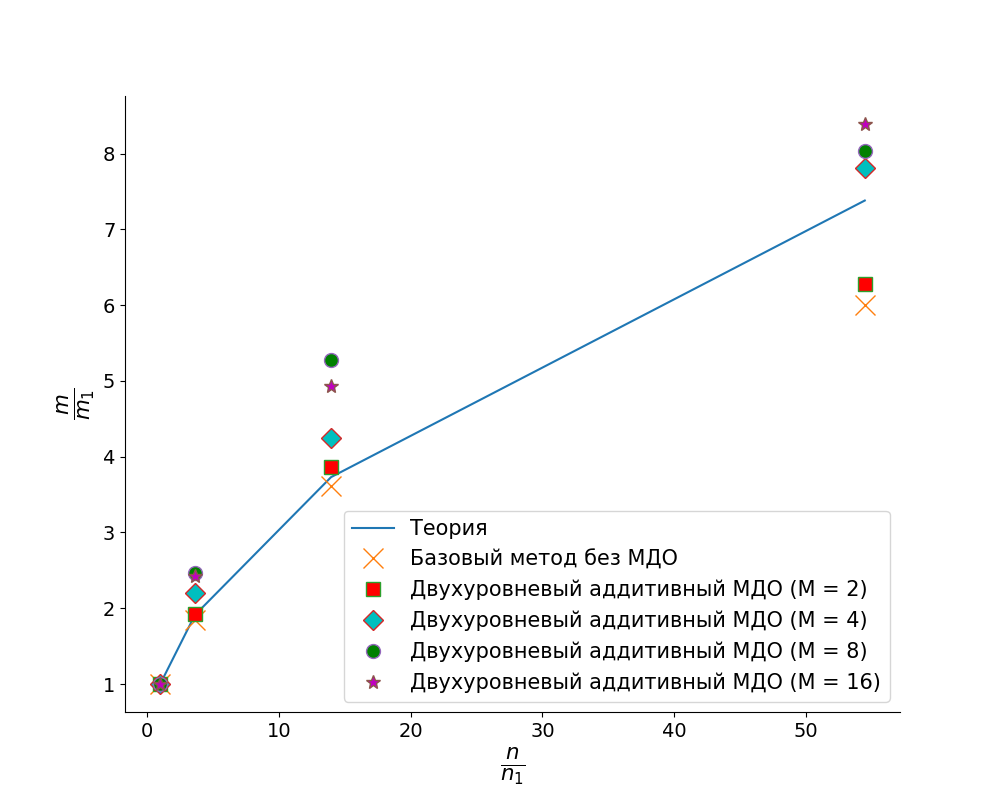
\includegraphics[scale=0.5]{../results/\area/\task/core/iters_cg.png}}
\caption{График отношений количества итераций}
\label{fig:task_\taskNum_iters_cg}
\end{figure}
\begin{figure}[H]
\center{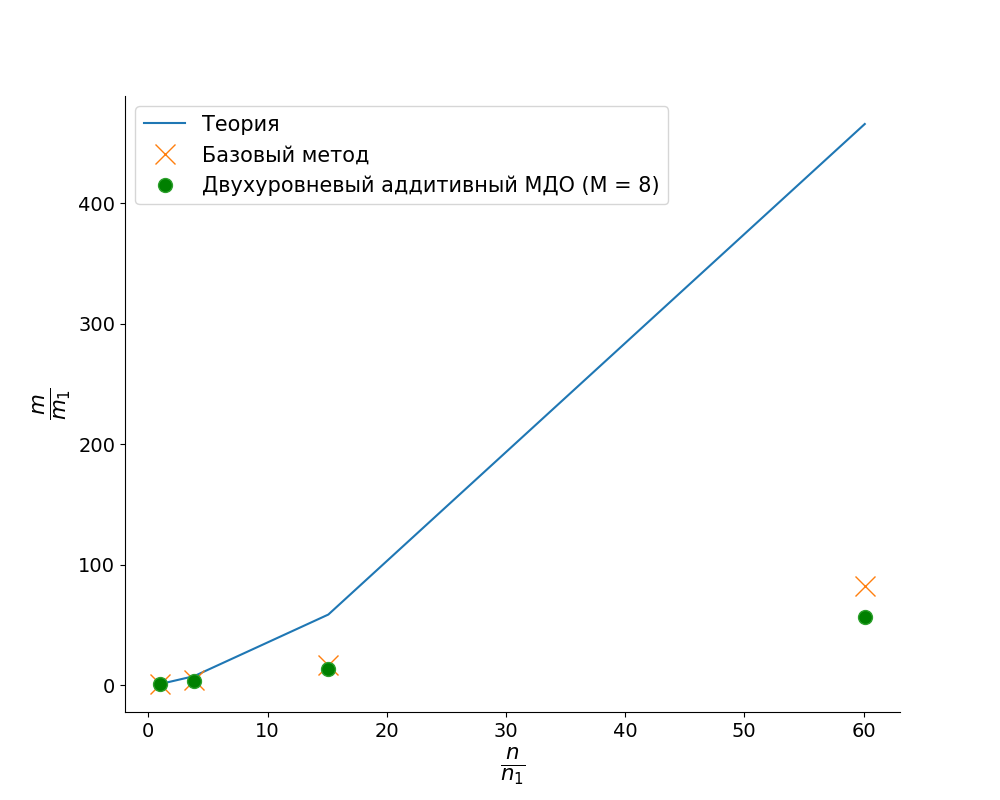
\includegraphics[scale=0.5]{../results/\area/\task/core/time_cg.png}}
\caption{График отношений временных затрат}
\label{fig:task_\taskNum_time_cg}
\end{figure}

\newpage

\subsection{Третья тестовая задача}

\renewcommand{\area}{thick_walled_cylinder}
\renewcommand{\task}{pressure_only}
\renewcommand{\taskNum}{03}

На рис. \ref{fig:task_\taskNum_scheme} представлена расчётная область - сектор поперечного сечения толстостенной трубы, нагруженной внешним давлением $p = 5$ МПа. Внутренний угол $\phi = 90$, внутренний радиус $p_a = 1$ см, внешний радиус $p_b = 2 $ см.

\begin{figure}[h]
\center{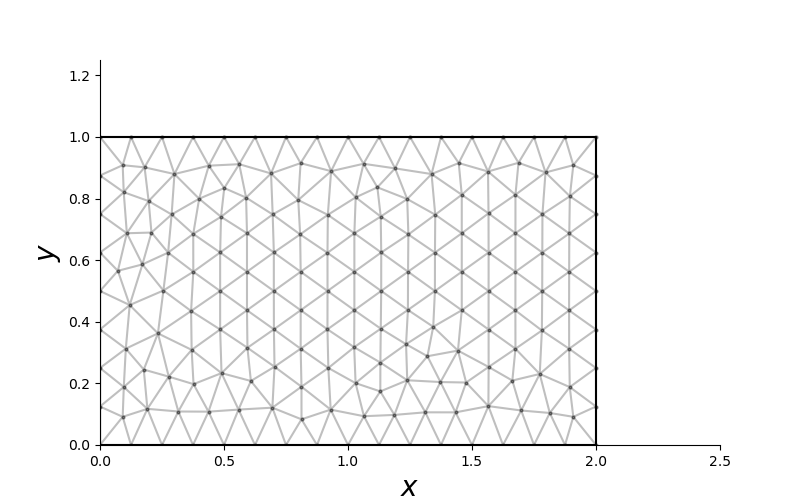
\includegraphics[scale=0.65]{../results/\area/\task/core/area_diagram.png}}
\caption{Схема расчётной области (h = 0.125)}
\label{fig:task_\taskNum_scheme}
\end{figure}

Для решения поставленной задачи примем, что материал тела имеет следующие параметры: модуль Юнга $E = 70$ ГПа, коэффициент Пуассона $\mu = 0.34$. 

Для исследования зависимости сходимости метода от размерности итоговой системы линейных уравнений рассмотрены три расчётные сетки с шагами $h = 0.05$ (количество узлов - 994), $h = 0.025$ (количество узлов - 3812), $h = 0.0125$ (количество узлов - 15006).

Для аддитивного метода Шварца итерационный параметр $\alpha = 0.5$.

\newpage

Для решения задачи методами декомпозиции области расчётная область разбивается по оси OX на заданное количество прямоугольных областей без перекрытия $\Omega_1, \ldots, \Omega_M$. Характерные размеры каждой подобласти: ширина подобласти $a_M = a / M$, высота подобласти совпадает с высотой тела $b_M = b$. На рис. \ref{fig:task_\taskNum_decomposition} представлена расчётная область первой тестовой задачи, разбитая на две подобласти.

\begin{figure}[h]
\center{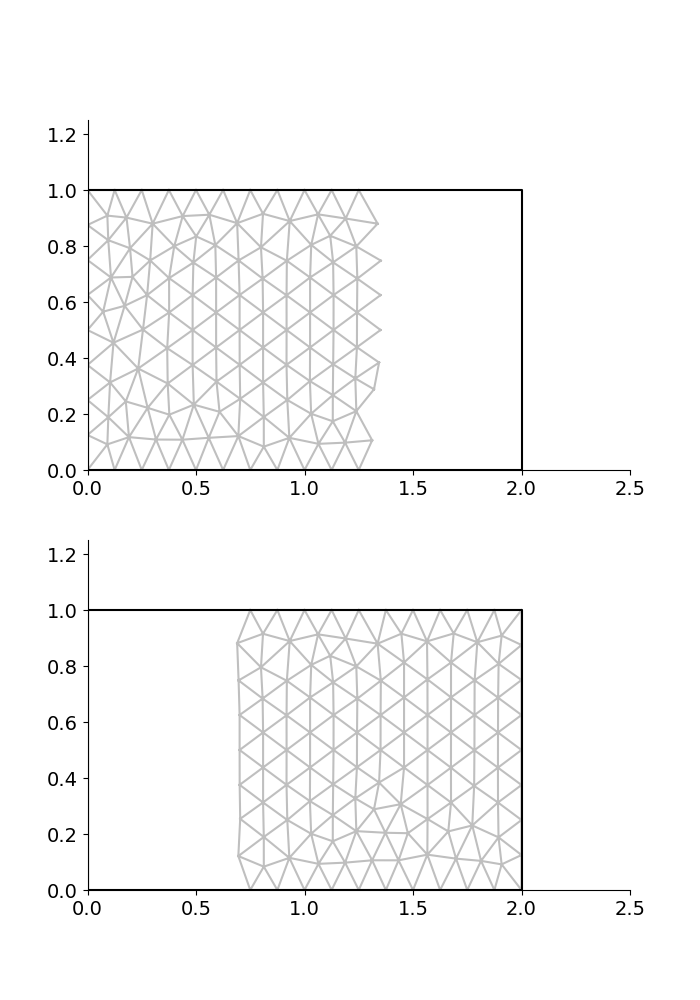
\includegraphics[scale=0.5]{../results/\area/\task/core/area_decomposition.png}}
\caption{Схема декомпозиции расчётной области (M = 2, h = 0.125)}
\label{fig:task_\taskNum_decomposition}
\end{figure}

\newpage

Для третьей тестовой задачи известно аналитическое решение для радиального перемещения и тензора напряжений $\left[6\right]$. Тогда аналитическое радиальное перемещение считаем по формуле:
\begin{equation*}
u_r = \frac{(1 + \mu) \cdot (1 - 2\mu)}{E}A \cdot r + \frac{(1 + \mu)}{E} \frac{B}{r},
\end{equation*}
где $A = (p_a \cdot r_a^2 - p_b \cdot r_b^2) / (r_b^2 - r_a^2)$, $B = (p_a - p_b) \cdot (r_a r_b)^2 / (r_b^2 - r_a^2)$.

Вычисление аналитического радиального и окружного напряжений производится по формуле:
\begin{equation*}
\sigma_{r, \varphi} = A \mp \frac{B}{r^2}
\end{equation*}

В таблице \ref{table:task_03_basic_errors} представлены относительные ошибки для третьей тестовой задачи, полученные методом без применения МДО для трёх разных шагов сетки, а в таблице \ref{table:task_03_basic_errors_rel} - отношения ошибок. Относительные ошибки вычислялись по формуле:
\begin{equation*}
\sqrt{\left(\sum_{k = 1}^{N_{elem}} {\left(\frac{\sigma_k^{ex} - \sigma_k^{num}}{\sigma_k^{ex}}\right)^2}\right) / \left(\sum_{k=1}^{N_{elem}} {s_k}\right)},
\end{equation*}

где $\sigma_k^{ex}$ - точное значение рассматриваемой компоненты тензора напряжений в центре k-ого элемента, $\sigma_k^{num}$ - полученное численное значение аналогичной величины, $s_k$ - площадь k-го элемента сетки. 

\newpage

Из таблицы \ref{table:task_\taskNum_basic_errors_rel} видно, что для напряжений наблюдается линейная скорость сходимости численного решения к аналитическому при измельчении сетки, для перемещений - квадратичная.
\begin{table}[h]
\caption{Ошибки численного решения в зависимости от шага сетки}
\csvloop{
	file = ../results/thick_walled_cylinder/pressure_only/core/errors.csv,
	head to column names,
	before reading = \centering\sisetup{table-number-alignment=center},
	tabular = {
		@{} |
		c |
		c | 
		c |
		c |
		@{}
	},
	table head = \hline Шаг сетки & \text{$u_r$} & \text{$\sigma_r$} & \text{$\sigma_\varphi$} \\\hline,
	command = \step & \ur & \sigmar & \sigmaphi,
	late after line = \\\hline
}
\label{table:task_\taskNum_basic_errors}
\end{table}

\begin{table}[h]
\caption{Отношение ошибок численного решения}
\csvloop{
	file = ../results/thick_walled_cylinder/pressure_only/core/errors_rel.csv,
	head to column names,
	before reading = \centering\sisetup{table-number-alignment=center},
	tabular = {
		@{} |
		c |
		c | 
		c |
		c |
		@{}
	},
	table head = \hline Шаг сетки & \text{$u_r$} & \text{$\sigma_r$} & \text{$\sigma_\varphi$} \\\hline,
	command = \step & \ur & \sigmar & \sigmaphi,
	late after line = \\\hline
}
\label{table:task_\taskNum_basic_errors_rel}
\end{table}

\newpage

На рис. \ref{fig:task_\taskNum_basic_displacement_distribution} приведено распределение радиальных перемещений, полученных при решении задачи во всей расчётной области базовым методом, на рис. \ref{fig:task_\taskNum_basic_pressure_distribution_r} и \ref{fig:task_\taskNum_basic_pressure_distribution_phi} - распределение узловых радиальных и окружных напряжений, полученных при решении задачи во всей расчётной области.

\begin{figure}[h]
\center{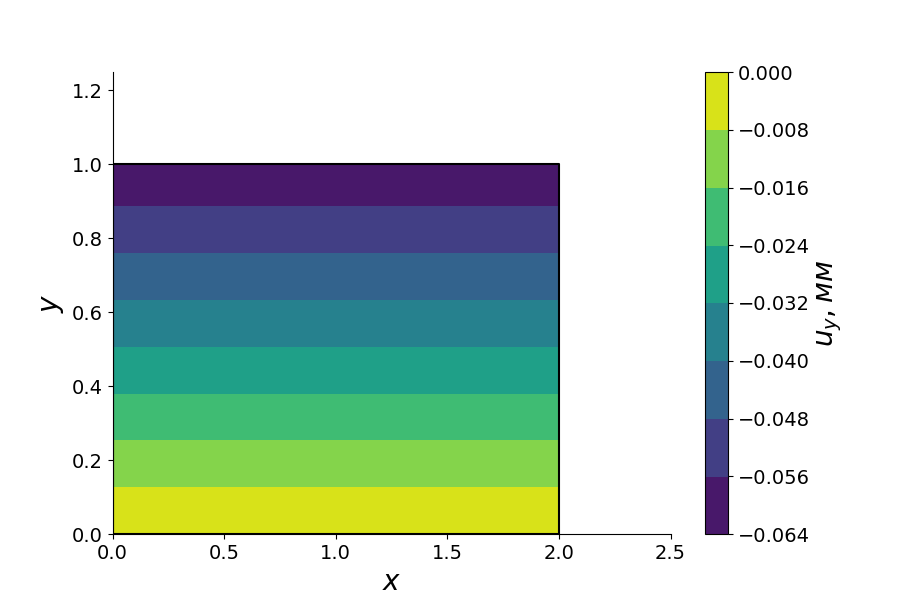
\includegraphics[scale=0.55]{../results/\area/\task/core/displacement_distribution.png}}
\caption{Распределение перемещений во всей расчётной области (h = 0.125)}
\label{fig:task_\taskNum_basic_displacement_distribution}
\end{figure}

\newpage

\begin{figure}[H]
\center{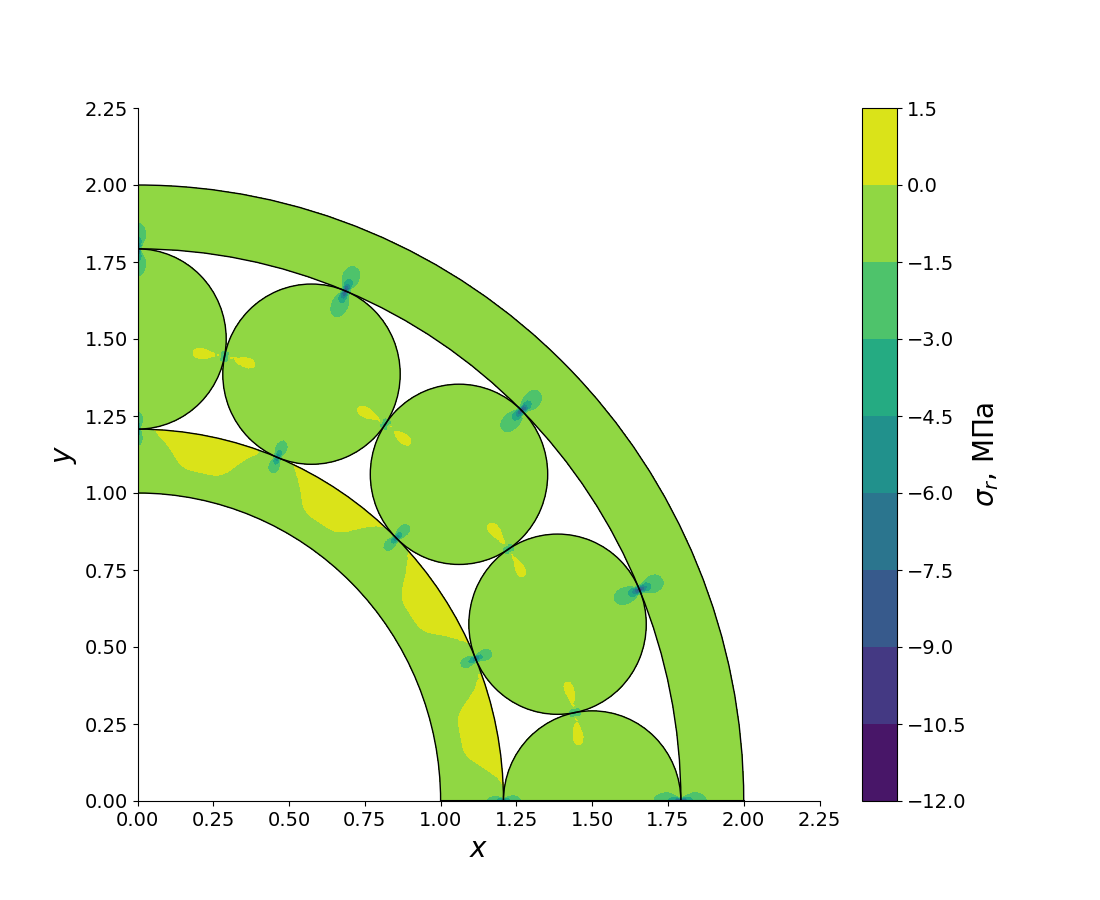
\includegraphics[scale=0.45]{../results/\area/\task/core/pressure_distribution_r.png}}
\caption{Распределение узловых радиальных напряжений во всей расчётной области (h = 0.0125)}
\label{fig:task_\taskNum_basic_pressure_distribution_r}
\end{figure}
\begin{figure}[H]
\center{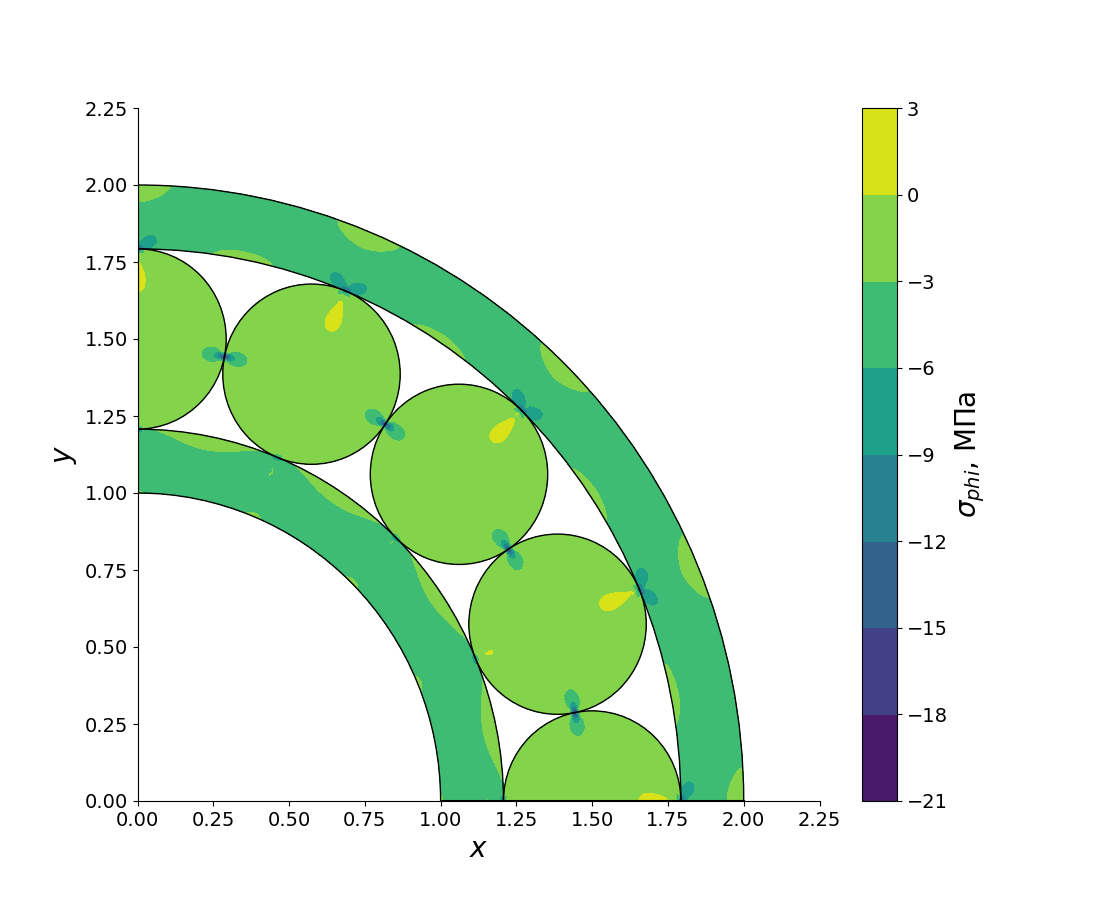
\includegraphics[scale=0.45]{../results/\area/\task/core/pressure_distribution_phi.png}}
\caption{Распределение узловых угловых напряжений во всей расчётной области (h = 0.0125)}
\label{fig:task_\taskNum_basic_pressure_distribution_phi}
\end{figure}

\newpage

\subsubsection{Мультипликативный метод Шварца}

В таблице \ref{table:task_\taskNum_mult_iters} представлено количество итераций в зависимости от количества подобластей и шага сетки при использовании мультипликативного метода Шварца (коэффициент захлёста для подобластей равен 0.3). Анализ полученных результатов показал, что:
\begin{itemize}
\item количество итераций не зависит от шага сетки;
\item при увеличении числа подобластей количество итераций увеличивается (при увеличении количества подобластей количество итераций увеличивается примерно в $M^2$ раз);
\end{itemize}

\begin{table}[h]
\caption{Количество итераций в зависимости от количества подобластей и шага сетки}
\csvloop{
	file = ../results/\area/\task/schwarz_multiplicative/iters.csv,
	head to column names,
	before reading = \centering\sisetup{table-number-alignment=center},
	tabular = {
		@{} |
		p{3cm} |
		c | 
		c |
		c |
		c |
		@{}
	},
	table head = \hline Количество подобластей (M) & \text{h = 0.05} & \text{h = 0.025} & \text{h = 0.0125} & \text{h = 0.00625} \\\hline,
	command = \amnt & \0 & \1 & \2 & \3,
	late after line = \\\hline
}
\label{table:task_\taskNum_mult_iters}
\end{table}

\newpage

\subsubsection{Аддитивный метод Шварца}

В таблице \ref{table:task_\taskNum_add_iters} представлено количество итераций в зависимости от количества подобластей и шага сетки при использовании аддитивного метода Шварца (коэффициент захлёста для подобластей равен 0.3). Анализ полученных результатов показал, что:
\begin{itemize}
\item количество итераций несильно зависит от шага сетки;
\item при увеличении числа подобластей количество итераций увеличивается (при увеличении количества подобластей количество итераций увеличивается примерно в $M^2$ раз);
\item количество итераций по сравнению со случаем применения мультипликативного метода Шварца выросло почти в 4 раза;
\end{itemize}

\begin{table}[h]
\caption{Количество итераций в зависимости от количества подобластей и шага сетки}
\csvloop{
	file = ../results/\area/\task/schwarz_additive/iters.csv,
	head to column names,
	before reading = \centering\sisetup{table-number-alignment=center},
	tabular = {
		@{} |
		p{3cm} |
		c | 
		c |
		c |
		c |
		@{}
	},
	table head = \hline Количество подобластей (M) & \text{h = 0.05} & \text{h = 0.025} & \text{h = 0.0125} & \text{h = 0.00625} \\\hline,
	command = \amnt & \0 & \1 & \2 & \3,
	late after line = \\\hline
}
\label{table:task_\taskNum_add_iters}
\end{table}

\newpage

\subsubsection{Двухуровневый аддитивный метод Шварца}

Для двухуровневого аддитивного метода кроме основной сетки в расчётной области зададим грубую сетку, удовлетворяющую условиям включения всех узлов мелкой сетки в элементы грубой сетки и соответствия размеров областей. 

Возьмём для нашей области в качестве грубой области сектор поперечного сечения цилиндра. Внутренний угол $\phi = 90$, внешний радиус $p_b = 2 $ см. На рис. \ref{fig:task_\taskNum_area_coarse_simplified_cylinder} изображена расчётная схема грубой области и узлы основной области.

\begin{figure}[h]
\center{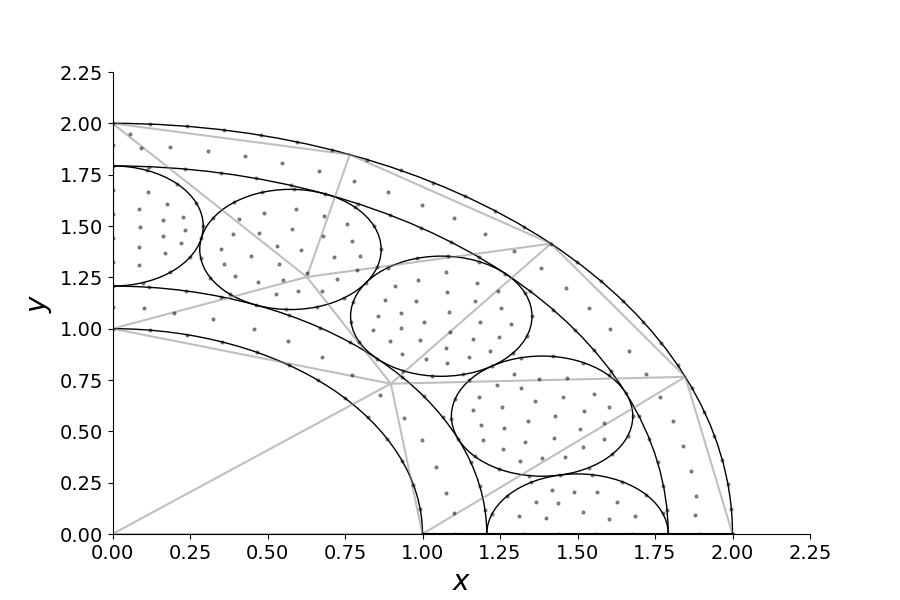
\includegraphics[scale=0.7]{../results/\area/\task/core/area_coarse_simplified_cylinder.png}}
\caption{Схема расчётной области с цилиндром в качестве грубой области (h = 0.125, H = 1)}
\label{fig:task_\taskNum_area_coarse_simplified_cylinder}
\end{figure}

\newpage

В таблице \ref{table:task_\taskNum_add2_coarse_simplified_cylinder} представлено количество итераций в зависимости от количества подобластей и шага грубой сетки при использовании двухуровневого аддитивного метода Шварца для шага мелкой сетки h = 0.0125 и взятого в качестве грубой области цилиндра (коэффициент захлёста для подобластей равен 0.3).

\begin{table}[h]
\caption{Количество итераций в зависимости от количества подобластей и шага грубой сетки для двухуровневого аддитивного метода Шварца для (h = 0.0125)}
\csvloop{
	file = ../results/\area/\task/schwarz_two_level_additive/iters_simplified_cylinder.csv,
	head to column names,
	before reading = \centering\sisetup{table-number-alignment=center},
	tabular = {
		@{} |
		c |
		c | 
		c |
		c |
		c |
		@{}
	},
	table head = \hline Количество подобластей & \text{H = 1} & \text{H = 0.5} & \text{H = 0.025} & \text{H = 0.125} \\\hline,
	command = \amnt & \0 & \1 & \2 & \3,
	late after line = \\\hline
}
\label{table:task_\taskNum_add2_coarse_simplified_cylinder}
\end{table}

Анализ данной таблицы показывает, что количество итераций довольно сильно зависит от количества подобластей даже при последовательном уменьшении шага грубой сетки. Поперечный сектор сечения цилиндра в качестве грубой области не подходит.

\newpage

Возьмём для нашей области в качестве грубой области сектор поперечного сечения толстостенной трубы. Внутренний угол $\phi = 90$, внутренний радиус $p_a = 1$ см, внешний радиус $p_b = 2 $ см. На рис. \ref{fig:task_\taskNum_area_coarse_thick_walled_cylinder} изображена расчётная схема грубой области и узлы основной области. На рис. \ref{fig:task_\taskNum_area_coarse_thick_walled_cylinder} изображена расчётная схема грубой области и узлы основной области.

\begin{figure}[h]
\center{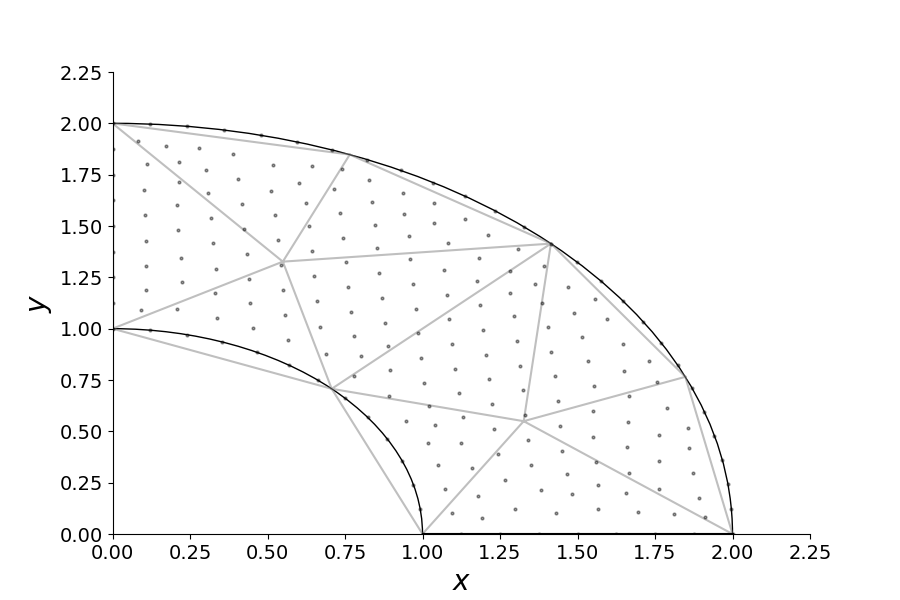
\includegraphics[scale=0.5]{../results/\area/\task/core/area_coarse_thick_walled_cylinder.png}}
\caption{Схема расчётной области с толстостенной трубой в качестве грубой области (h = 0.125, H = 1)}
\label{fig:task_\taskNum_area_coarse_thick_walled_cylinder}
\end{figure}

В таблице \ref{table:task_\taskNum_add2_coarse_thick_walled_cylinder} представлено количество итераций в зависимости от количества подобластей и шага грубой сетки при использовании двухуровневого аддитивного метода Шварца для шага мелкой сетки h = 0.0125 и взятой в качестве грубой области толстостенной трубы (коэффициент захлёста для подобластей равен 0.3).

Анализ данной таблицы показывает, что для расчётов рациональнее взять шаг H = 0.125, так как в этом случае количество итераций незначительно зависит от количества подобластей.

\newpage

\begin{table}[h]
\caption{Количество итераций в зависимости от количества подобластей и шага грубой сетки для двухуровневого аддитивного метода Шварца (h = 0.0125)}
\csvloop{
	file = ../results/\area/\task/schwarz_two_level_additive/iters_thick_walled_cylinder.csv,
	head to column names,
	before reading = \centering\sisetup{table-number-alignment=center},
	tabular = {
		@{} |
		c |
		c | 
		c |
		c |
		@{}
	},
	table head = \hline Количество подобластей & \text{H = 0.5} & \text{H = 0.025} & \text{H = 0.125} \\\hline,
	command = \amnt & \0 & \1 & \2,
	late after line = \\\hline
}
\label{table:task_\taskNum_add2_coarse_thick_walled_cylinder}
\end{table}

В таблице \ref{table:task_\taskNum_add2_iters} представлено количество итераций в зависимости от количества подобластей и шага сетки при использовании двухуровневого аддитивного метода Шварца для первой тестовой задачи при H = 0.125 (коэффициент захлёста для подобластей равен 0.3). Анализ полученных результатов показал, что:
\begin{itemize}
\item количество итераций не зависит от шага сетки;
\item при увеличении числа подобластей количество итераций не меняется;
\end{itemize}

\begin{table}[h]
\caption{Количество итераций в зависимости от количества подобластей и шага сетки для двухуровневого аддитивного метода Шварца (H = 0.125)}
\csvloop{
	file = ../results/\area/\task/schwarz_two_level_additive/iters.csv,
	head to column names,
	before reading = \centering\sisetup{table-number-alignment=center},
	tabular = {
		@{} |
		c |
		c | 
		c |
		c |
		c |
		@{}
	},
	table head = \hline Количество подобластей & \text{h = 0.05} & \text{h = 0.025} & \text{h = 0.0125} & \text{h = 0.00625} \\\hline,
	command = \amnt & \0 & \1 & \2 & \3,
	late after line = \\\hline
}
\label{table:task_\taskNum_add2_iters}
\end{table}

В таблице \ref{table:task_\taskNum_iters_overlap} рассмотрена зависимость количества итераций от различных вариантов МДО и коэффициента относительного захлёста при M = 4, h = 0.025 и H = 0.125. Из таблицы видно, что при росте коэффициента относительного захлёста количество итераций уменьшается.

\begin{table}[h]
\caption{Количество итераций в зависимости от метода декомпозиции области и коэффициента относительного захлёста (M = 4, h = 0.025, H = 0.125)}
\csvloop{
	file = ../results/\area/\task/core/iters_overlap.csv,
	head to column names,
	before reading = \centering\sisetup{table-number-alignment=center},
	tabular = {
		@{} |
		c |
		c |
		c |
		c |
		@{}
	},
	table head = \hline Коэффициент относительного захлёста & 0.2 & 0.3 & 0.4 \\\hline,
	command = \method & \0 & \1 & \2,
	late after line = \\\hline
}
\label{table:task_\taskNum_iters_overlap}
\end{table}

\newpage
В таблице \ref{table:task_\taskNum_iters_cg} приведены количество итераций, за которое сходится метод сопряженных градиентов, при решении задачи во всей области без методов декомпозиции, а также общее количество итераций, за которое сходится метода сопряженных градиентов для каждой локальной задачи, при решении задачи во всей области двухуровневым аддитивным методом Шварца.

В таблице \ref{table:task_\taskNum_iters_cg_rel} приведены отношения размерностей систем, отношения количества итераций при решении задачи во всей области без методов декомпозиции, отношения количества итераций в соответствии с теорией и отношения количества итераций при решении задачи во всей области двухуровневым аддитивным методом Шварца.

Из таблицы \ref{table:task_\taskNum_iters_cg_rel} видно, что отношения для базового метода и двухуровневого метода практически идентичны благодаря тому, что общее количество итераций для двухуровневого аддитивного метода Шварца не меняется при изменении размерности системы. На рис. \ref{fig:task_01_iters_cg} наглядно продемонстрированы результаты, полученные в таблице \ref{table:task_\taskNum_iters_cg_rel}.

\begin{table}[h]
\caption{Количество итераций метода сопряженных градиентов в зависимости от размера СЛАУ и метода решения задачи}
\csvloop{
	file = ../results/\area/\task/core/iters_cg.csv,
	head to column names,
	before reading = \centering\sisetup{table-number-alignment=center},
	tabular = {
		@{} |
		c |
		c |
		c |
		@{}
	},
	table head = \hline Размерность системы & Базовый метод & Двухуровневый аддитивный МДО \\\hline,
	command = \index & \basic & \8,
	late after line = \\\hline
}
\label{table:task_\taskNum_iters_cg}
\end{table}

\begin{table}[h]
\caption{Отношение количества итераций метода сопряженных градиентов}
\csvloop{
	file = ../results/\area/\task/core/iters_cg_rel.csv,
	head to column names,
	before reading = \centering\sisetup{table-number-alignment=center},
	tabular = {
		@{} |
		p{3.0cm} |
		p{3.0cm} |
		l |
		l |
		p{4.0cm} |
		@{}
	},
	table head = \hline Размерность системы & Отношение размеров & Теория & Базовый метод & Двухуровневый аддитивный МДО \\\hline,
	command = \index & \N & \theory & \basic & \8,
	late after line = \\\hline
}
\label{table:task_\taskNum_iters_cg_rel}
\end{table}

\newpage

В таблице \ref{table:task_\taskNum_time_cg} приведены временные затраты, необходимые для решения задачи во всей области без методов декомпозиции, а также временные затраты для решения задачи во всей области двухуровневым аддитивным методом Шварца.

В таблице \ref{table:task_\taskNum_time_cg_rel} приведены отношения размерностей систем, отношения временных затрат при решении задачи во всей области без методов декомпозиции, отношения временных затрат в соответствии с теорией и отношения временных затрат при решении задачи во всей области двухуровневым аддитивным методом Шварца.

Из таблицы \ref{table:task_\taskNum_time_cg_rel} видно, что отношение временных затрат для двухуровневого аддитивного метода Шварца лучше, чем для теоретического случая и тем более для базового метода решения задачи без применения МДО. На рис. \ref{fig:task_\taskNum_time_cg} наглядно продемонстрированы результаты, полученные в таблице \ref{table:task_\taskNum_time_cg_rel}.

\begin{table}[h]
\caption{Время, затраченное на метод сопряженных градиентов, в зависимости от размера СЛАУ и метода решения задачи}
\csvloop{
	file = ../results/\area/\task/core/time_cg.csv,
	head to column names,
	before reading = \centering\sisetup{table-number-alignment=center},
	tabular = {
		@{} |
		c |
		c |
		c |
		@{}
	},
	table head = \hline Размер СЛАУ & Базовый метод & Двухуровневый аддитивный МДО \\\hline,
	command = \index & \basic & \8,
	late after line = \\\hline
}
\label{table:task_\taskNum_time_cg}
\end{table}

\begin{table}[h]
\caption{Отношение затраченного времени на метод сопряженных градиентов}
\csvloop{
	file = ../results/\area/\task/core/time_cg_rel.csv,
	head to column names,
	before reading = \centering\sisetup{table-number-alignment=center},
	tabular = {
		@{} |
		p{3.0cm} |
		p{3.0cm} |
		l |
		l |
		p{4.0cm} |
		@{}
	},
	table head = \hline Размер СЛАУ & Теория & Базовый метод & Двухуровневый аддитивный МДО \\\hline,
	command = \index & \theory & \basic & \8,
	late after line = \\\hline
}
\label{table:task_\taskNum_time_cg_rel}
\end{table}

\newpage

\begin{figure}[H]
\center{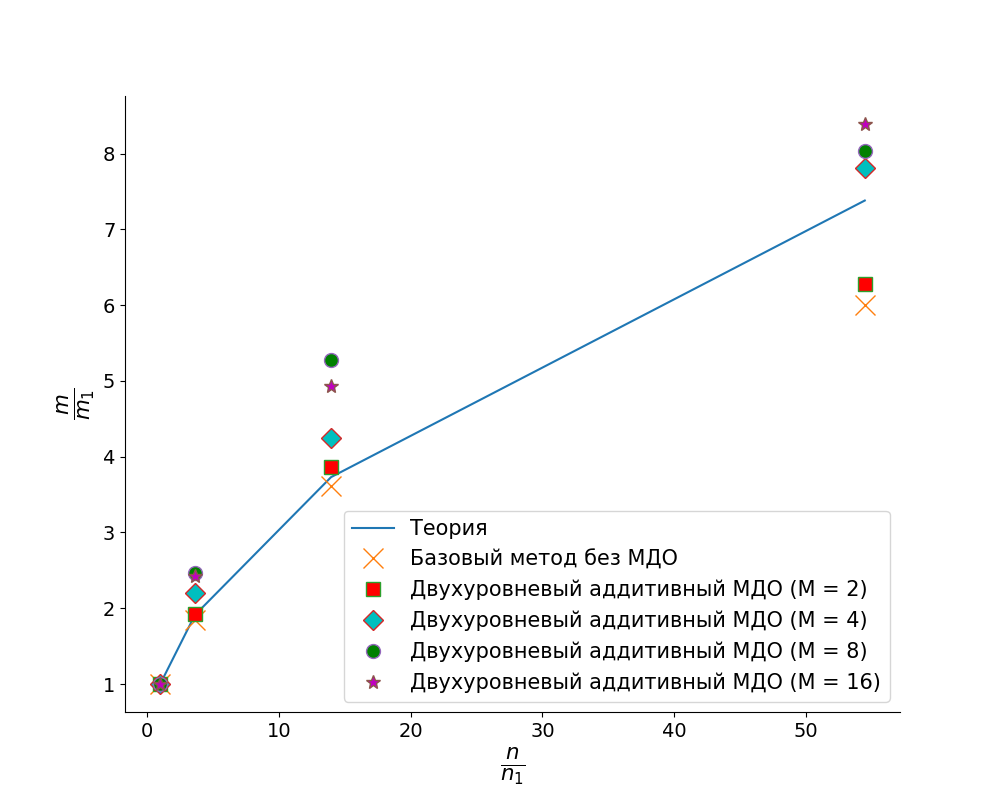
\includegraphics[scale=0.5]{../results/\area/\task/core/iters_cg.png}}
\caption{График отношений количества итераций}
\label{fig:task_\taskNum_iters_cg}
\end{figure}
\begin{figure}[H]
\center{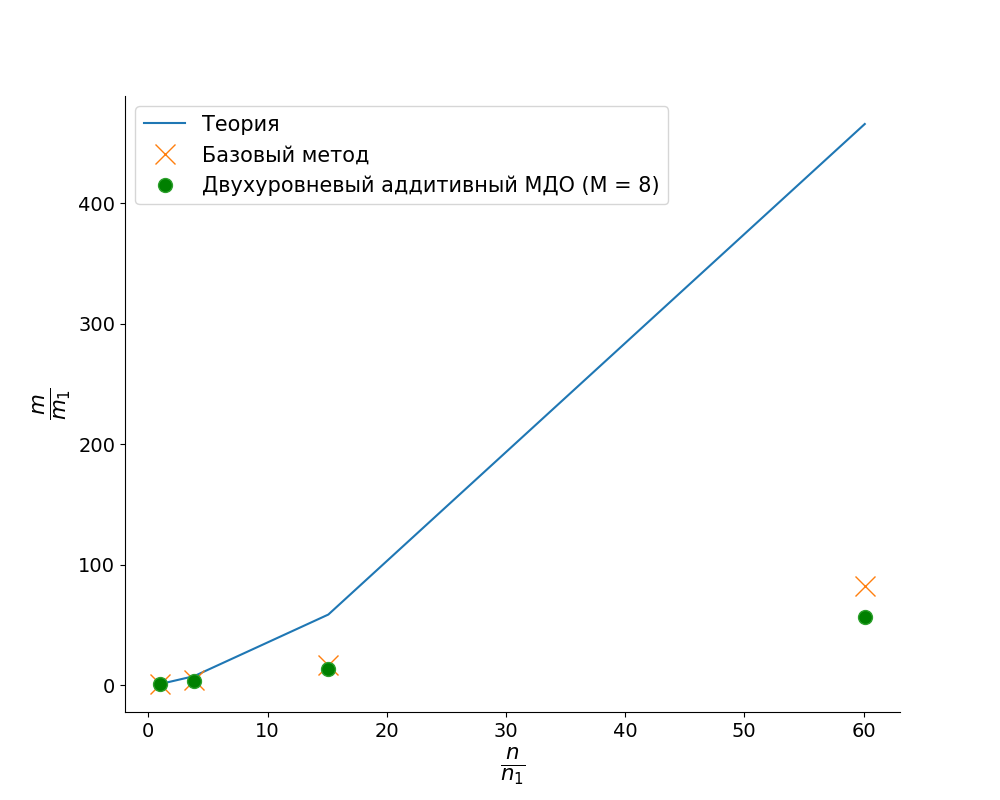
\includegraphics[scale=0.5]{../results/\area/\task/core/time_cg.png}}
\caption{График отношений временных затрат}
\label{fig:task_\taskNum_time_cg}
\end{figure}

\newpage

\subsection{Четвёртая тестовая задача}

\renewcommand{\area}{bearing}
\renewcommand{\task}{pressure_only}
\renewcommand{\taskNum}{04}

На рис. \ref{fig:task_\taskNum_scheme} представлена расчётная область - сектор поперечного сечения модели подшипника, нагруженной внешним давлением $p = 5$ МПа. Внутренний радиус $p_a = 1$ см, внешний радиус $p_b = 2 $ см.

\begin{figure}[h]
\center{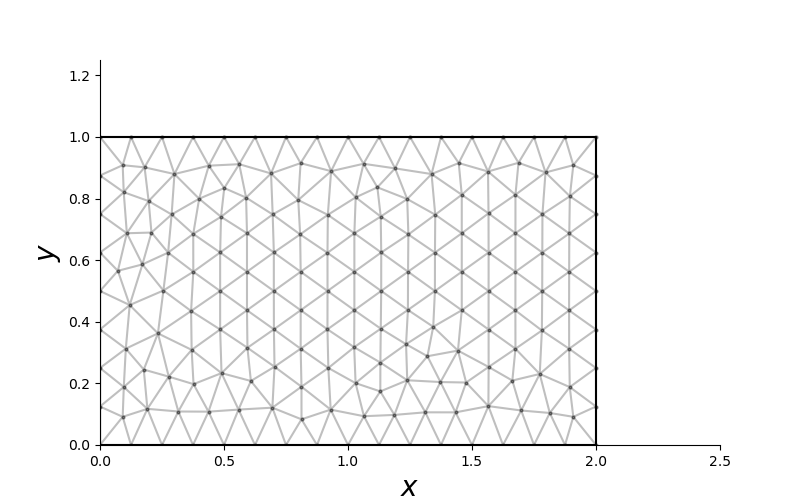
\includegraphics[scale=0.7]{../results/\area/\task/core/area_diagram.png}}
\caption{Схема расчётной области (h = 0.125)}
\label{fig:task_\taskNum_scheme}
\end{figure}

Для решения поставленной задачи примем, что материал тела имеет следующие параметры: модуль Юнга $E = 70$ ГПа, коэффициент Пуассона $\mu = 0.34$. 

Для исследования зависимости сходимости метода от размерности итоговой системы линейных уравнений рассмотрены три расчётные сетки с шагами $h = 0.05$ (количество узлов - 994), $h = 0.025$ (количество узлов - 3812), $h = 0.0125$ (количество узлов - 15006).

Для аддитивного метода Шварца итерационный параметр $\alpha = 0.5$.

\newpage

Для решения задачи методами декомпозиции области расчётная область разбивается по оси OX на заданное количество прямоугольных областей без перекрытия $\Omega_1, \ldots, \Omega_M$. Характерные размеры каждой подобласти: ширина подобласти $a_M = a / M$, высота подобласти совпадает с высотой тела $b_M = b$. На рис. \ref{fig:task_\taskNum_decomposition} представлена расчётная область первой тестовой задачи, разбитая на две подобласти.

\begin{figure}[h]
\center{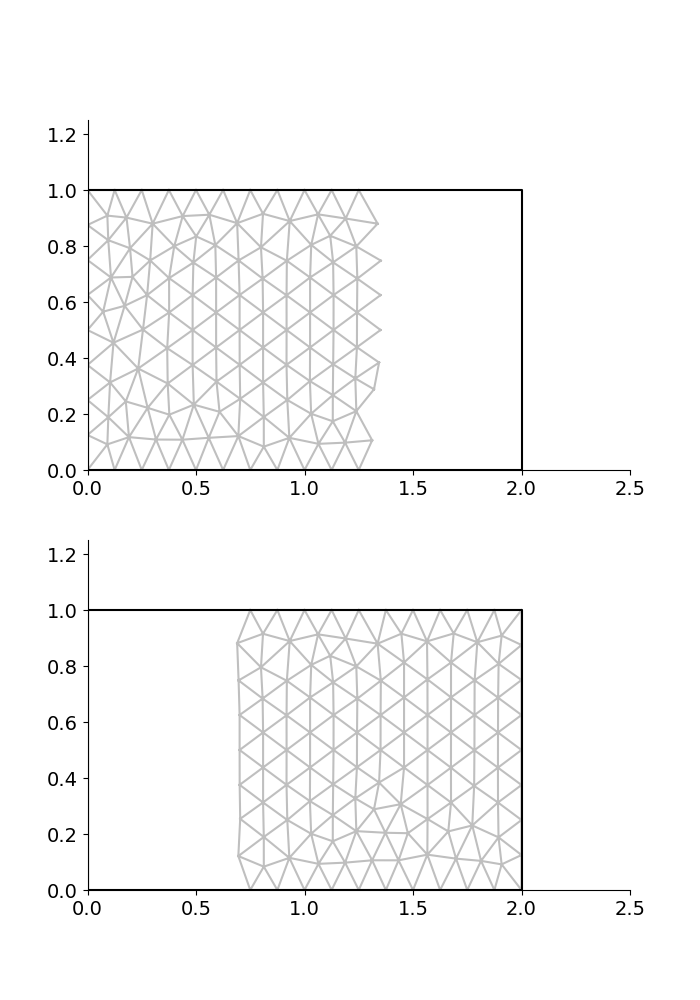
\includegraphics[scale=0.5]{../results/\area/\task/core/area_decomposition.png}}
\caption{Схема декомпозиции расчётной области (M = 2, h = 0.125)}
\label{fig:task_\taskNum_decomposition}
\end{figure}

\newpage

На рис. \ref{fig:task_\taskNum_basic_displacement_distribution} приведено распределение радиальных перемещений, полученных при решении задачи во всей расчётной области базовым методом, на рис. \ref{fig:task_\taskNum_basic_pressure_distribution_r} и \ref{fig:task_\taskNum_basic_pressure_distribution_phi} - распределение узловых радиальных и окружных напряжений, полученных при решении задачи во всей расчётной области.

\begin{figure}[h]
\center{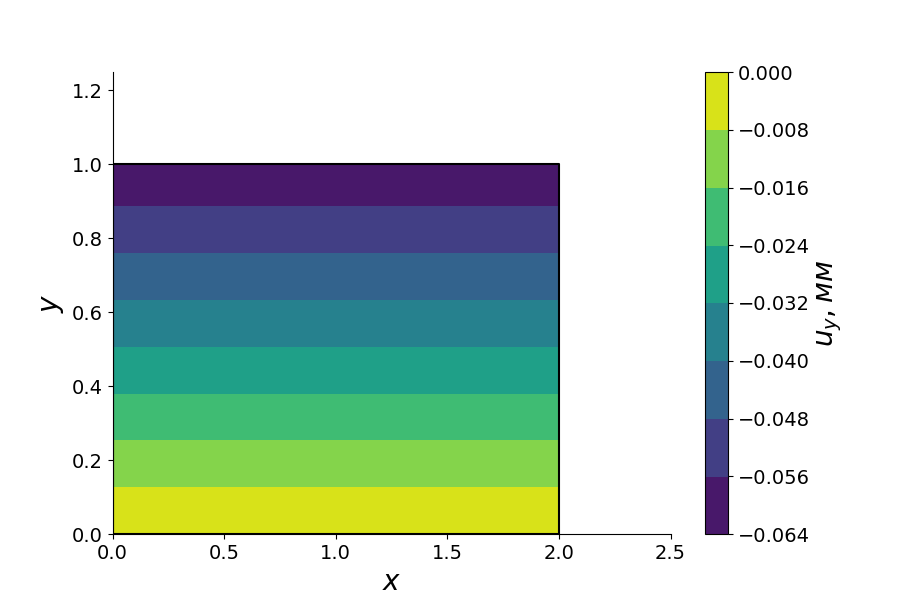
\includegraphics[scale=0.55]{../results/\area/\task/core/displacement_distribution.png}}
\caption{Распределение перемещений во всей расчётной области (h = 0.125)}
\label{fig:task_\taskNum_basic_displacement_distribution}
\end{figure}

\newpage

\begin{figure}[H]
\center{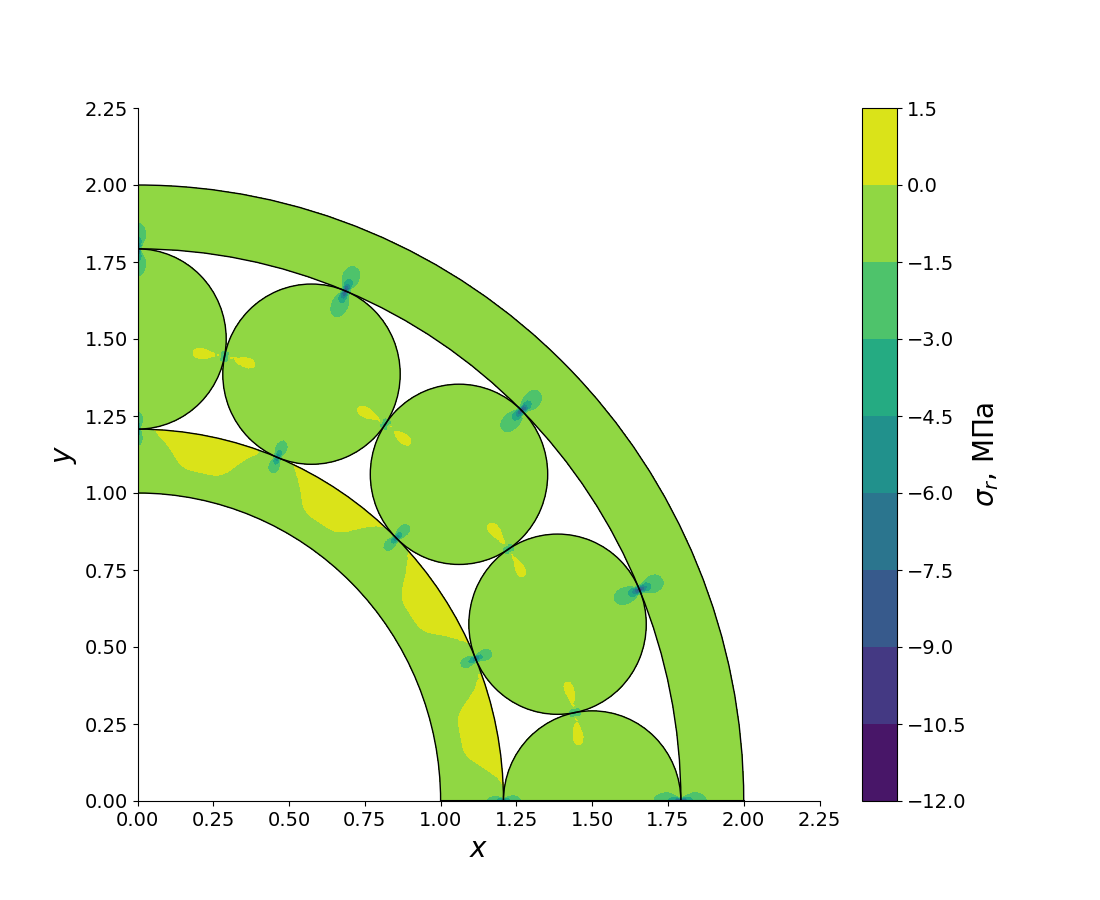
\includegraphics[scale=0.45]{../results/\area/\task/core/pressure_distribution_r.png}}
\caption{Распределение узловых радиальных напряжений во всей расчётной области (h = 0.0125)}
\label{fig:task_\taskNum_basic_pressure_distribution_r}
\end{figure}
\begin{figure}[H]
\center{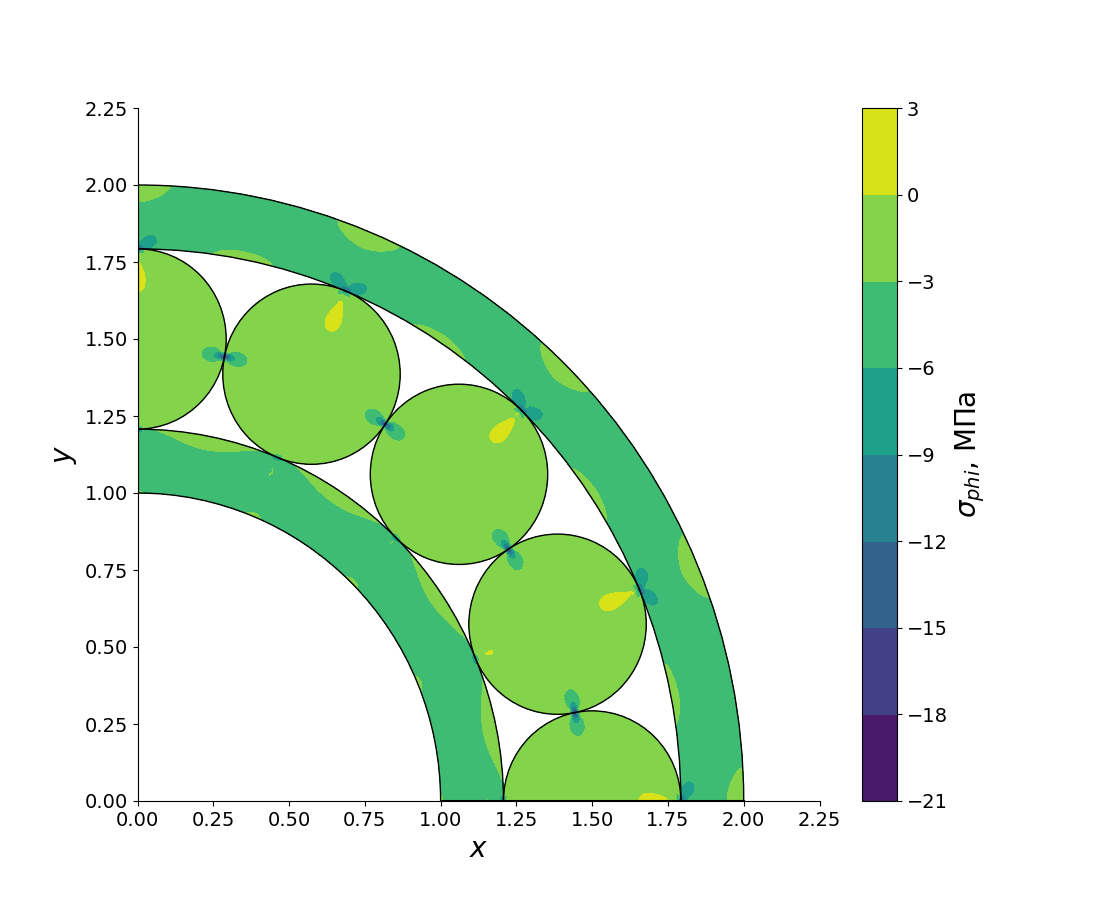
\includegraphics[scale=0.45]{../results/\area/\task/core/pressure_distribution_phi.png}}
\caption{Распределение узловых угловых напряжений во всей расчётной области (h = 0.0125)}
\label{fig:task_\taskNum_basic_pressure_distribution_phi}
\end{figure}

\newpage

\subsubsection{Мультипликативный метод Шварца}

В таблице \ref{table:task_\taskNum_mult_iters} представлено количество итераций в зависимости от количества подобластей и шага сетки при использовании мультипликативного метода Шварца (коэффициент захлёста для подобластей равен 0.3). Анализ полученных результатов показал, что:
\begin{itemize}
\item количество итераций не зависит от шага сетки;
\item при увеличении числа подобластей количество итераций увеличивается (при увеличении количества подобластей количество итераций увеличивается примерно в $M^2$ раз);
\end{itemize}

\begin{table}[h]
\caption{Количество итераций в зависимости от количества подобластей и шага сетки}
\csvloop{
	file = ../results/\area/\task/schwarz_multiplicative/iters.csv,
	head to column names,
	before reading = \centering\sisetup{table-number-alignment=center},
	tabular = {
		@{} |
		p{3cm} |
		c | 
		c |
		c |
		c |
		@{}
	},
	table head = \hline Количество подобластей (M) & \text{h = 0.05} & \text{h = 0.025} & \text{h = 0.0125} & \text{h = 0.00625} \\\hline,
	command = \amnt & \0 & \1 & \2 & \3,
	late after line = \\\hline
}
\label{table:task_\taskNum_mult_iters}
\end{table}

\newpage

\subsubsection{Аддитивный метод Шварца}

В таблице \ref{table:task_\taskNum_add_iters} представлено количество итераций в зависимости от количества подобластей и шага сетки при использовании аддитивного метода Шварца (коэффициент захлёста для подобластей равен 0.3). Анализ полученных результатов показал, что:
\begin{itemize}
\item количество итераций несильно зависит от шага сетки;
\item при увеличении числа подобластей количество итераций увеличивается (при увеличении количества подобластей количество итераций увеличивается примерно в $M^2$ раз);
\item количество итераций по сравнению со случаем применения мультипликативного метода Шварца выросло почти в 4 раза;
\end{itemize}

\begin{table}[h]
\caption{Количество итераций в зависимости от количества подобластей и шага сетки}
\csvloop{
	file = ../results/\area/\task/schwarz_additive/iters.csv,
	head to column names,
	before reading = \centering\sisetup{table-number-alignment=center},
	tabular = {
		@{} |
		p{3cm} |
		c | 
		c |
		c |
		c |
		@{}
	},
	table head = \hline Количество подобластей (M) & \text{h = 0.05} & \text{h = 0.025} & \text{h = 0.0125} & \text{h = 0.00625} \\\hline,
	command = \amnt & \0 & \1 & \2 & \3,
	late after line = \\\hline
}
\label{table:task_\taskNum_add_iters}
\end{table}

\newpage

\subsubsection{Двухуровневый аддитивный метод Шварца}

Для двухуровневого аддитивного метода кроме основной сетки в расчётной области зададим грубую сетку, удовлетворяющую условиям включения всех узлов мелкой сетки в элементы грубой сетки и соответствия размеров областей. 

Возьмём для нашей области в качестве грубой области сектор поперечного сечения цилиндра. Внутренний угол $\phi = 90$, внешний радиус $p_b = 2 $ см. На рис. \ref{fig:task_\taskNum_area_coarse_simplified_cylinder} изображена расчётная схема грубой области и узлы основной области.

\begin{figure}[h]
\center{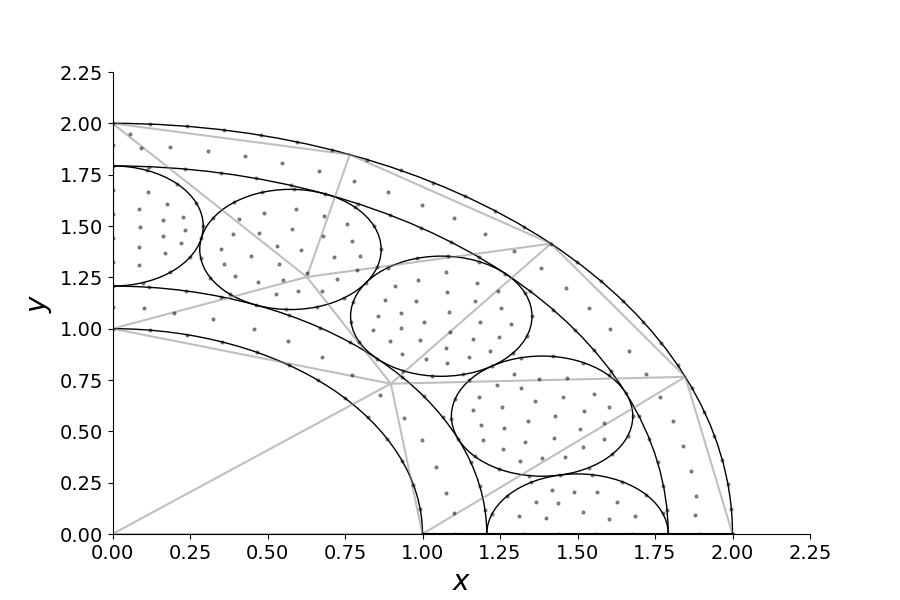
\includegraphics[scale=0.7]{../results/\area/\task/core/area_coarse_simplified_cylinder.png}}
\caption{Схема расчётной области с цилиндром в качестве грубой области (h = 0.125, H = 1)}
\label{fig:task_\taskNum_area_coarse_simplified_cylinder}
\end{figure}

\newpage

В таблице \ref{table:task_\taskNum_add2_coarse_simplified_cylinder} представлено количество итераций в зависимости от количества подобластей и шага грубой сетки при использовании двухуровневого аддитивного метода Шварца для шага мелкой сетки h = 0.0125 и взятого в качестве грубой области цилиндра (коэффициент захлёста для подобластей равен 0.3).

\begin{table}[h]
\caption{Количество итераций в зависимости от количества подобластей и шага грубой сетки для двухуровневого аддитивного метода Шварца для (h = 0.0125)}
\csvloop{
	file = ../results/\area/\task/schwarz_two_level_additive/iters_simplified_cylinder.csv,
	head to column names,
	before reading = \centering\sisetup{table-number-alignment=center},
	tabular = {
		@{} |
		c |
		c | 
		c |
		c |
		c |
		@{}
	},
	table head = \hline Количество подобластей & \text{H = 1} & \text{H = 0.5} & \text{H = 0.025} & \text{H = 0.125} \\\hline,
	command = \amnt & \0 & \1 & \2 & \3,
	late after line = \\\hline
}
\label{table:task_\taskNum_add2_coarse_simplified_cylinder}
\end{table}

Анализ данной таблицы показывает, что количество итераций довольно сильно зависит от количества подобластей даже при последовательном уменьшении шага грубой сетки. Поперечный сектор сечения цилиндра в качестве грубой области не подходит.

\newpage

Возьмём для нашей области в качестве грубой области сектор поперечного сечения толстостенной трубы. Внутренний угол $\phi = 90$, внутренний радиус $p_a = 1 $ см, внешний радиус $p_b = 2 $ см. На рис. \ref{fig:task_\taskNum_area_coarse_thick_walled_cylinder} изображена расчётная схема грубой области и узлы основной области.

\begin{figure}[h]
\center{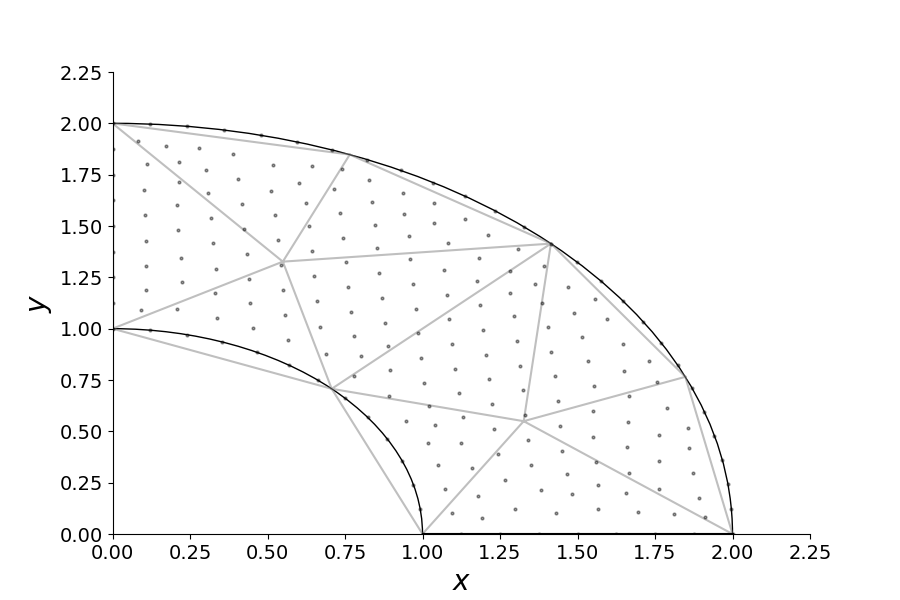
\includegraphics[scale=0.7]{../results/\area/\task/core/area_coarse_thick_walled_cylinder.png}}
\caption{Схема расчётной области с толстостенной трубой в качестве грубой области (h = 0.125, H = 1)}
\label{fig:task_\taskNum_area_coarse_thick_walled_cylinder}
\end{figure}

\newpage

В таблице \ref{table:task_\taskNum_add2_coarse_thick_walled_cylinder} представлено количество итераций в зависимости от количества подобластей и шага грубой сетки при использовании двухуровневого аддитивного метода Шварца для шага мелкой сетки h = 0.0125 и взятой в качестве грубой области толстостенной трубы (коэффициент захлёста для подобластей равен 0.3).

\begin{table}[h]
\caption{Количество итераций в зависимости от количества подобластей и шага грубой сетки для двухуровневого аддитивного метода Шварца для (h = 0.0125)}
\csvloop{
	file = ../results/\area/\task/schwarz_two_level_additive/iters_thick_walled_cylinder.csv,
	head to column names,
	before reading = \centering\sisetup{table-number-alignment=center},
	tabular = {
		@{} |
		c |
		c | 
		c |
		c |
		c |
		@{}
	},
	table head = \hline Количество подобластей & \text{H = 1} & \text{H = 0.5} & \text{H = 0.025} & \text{H = 0.125} \\\hline,
	command = \amnt & \0 & \1 & \2 & \3,
	late after line = \\\hline
}
\label{table:task_\taskNum_add2_coarse_thick_walled_cylinder}
\end{table}

Анализ данной таблицы показывает, что количество итераций довольно сильно зависит от количества подобластей даже при последовательном уменьшении шага грубой сетки. Поперечный сектор сечения толстостенной трубы в качестве грубой области не подходит.

\newpage

Возьмём для нашей области в качестве грубой области сектор поперечного сечения модели подшипника. Внутренний угол $\phi = 90$, внутренний радиус $p_a = 1$ см, внешний радиус $p_b = 2 $ см. На рис. \ref{fig:task_\taskNum_area_coarse_thick_walled_cylinder} изображена расчётная схема грубой области и узлы основной области. На рис. \ref{fig:task_\taskNum_area_coarse_thick_walled_cylinder} изображена расчётная схема грубой области и узлы основной области.

\begin{figure}[h]
\center{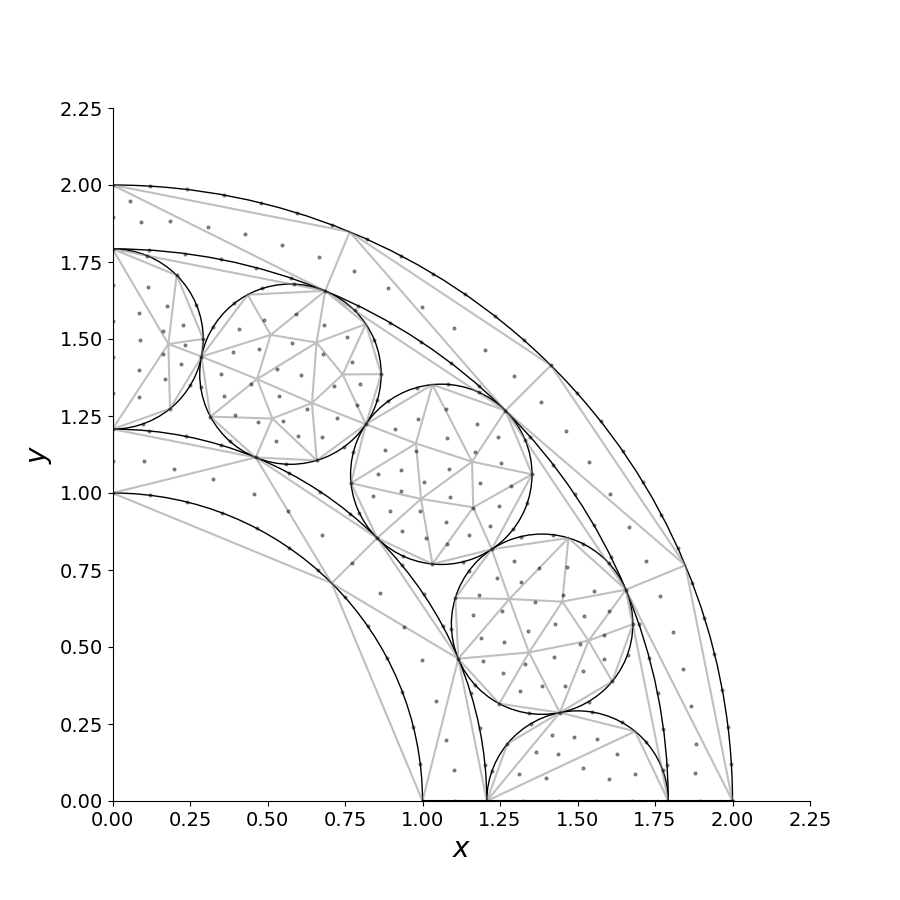
\includegraphics[scale=0.6]{../results/\area/\task/core/area_coarse_bearing.png}}
\caption{Схема расчётной области с моделью подшипника в качестве грубой области (h = 0.125, H = 1)}
\label{fig:task_\taskNum_area_coarse_bearing}
\end{figure}

В таблице \ref{table:task_\taskNum_add2_coarse_bearing} представлено количество итераций в зависимости от количества подобластей и шага грубой сетки при использовании двухуровневого аддитивного метода Шварца для шага мелкой сетки h = 0.0125 и взятой в качестве грубой области модели подшипника (коэффициент захлёста для подобластей равен 0.3). Анализ данной таблицы показывает, что для расчётов рациональнее взять шаг H = 0.125, так как в этом случае количество итераций незначительно зависит от количества подобластей.

\newpage

\begin{table}[h]
\caption{Количество итераций в зависимости от количества подобластей и шага грубой сетки для двухуровневого аддитивного метода Шварца (h = 0.0125)}
\csvloop{
	file = ../results/\area/\task/schwarz_two_level_additive/iters_bearing.csv,
	head to column names,
	before reading = \centering\sisetup{table-number-alignment=center},
	tabular = {
		@{} |
		c |
		c | 
		c |
		c |
		@{}
	},
	table head = \hline Количество подобластей & \text{H = 0.5} & \text{H = 0.025} & \text{H = 0.125} \\\hline,
	command = \amnt & \0 & \1 & \2,
	late after line = \\\hline
}
\label{table:task_\taskNum_add2_coarse_bearing}
\end{table}

В таблице \ref{table:task_\taskNum_add2_iters} представлено количество итераций в зависимости от количества подобластей и шага сетки при использовании двухуровневого аддитивного метода Шварца для первой тестовой задачи при H = 0.125 (коэффициент захлёста для подобластей равен 0.3). Анализ полученных результатов показал, что:
\begin{itemize}
\item количество итераций не зависит от шага сетки;
\item при увеличении числа подобластей количество итераций не меняется;
\end{itemize}

\begin{table}[h]
\caption{Количество итераций в зависимости от количества подобластей и шага сетки для двухуровневого аддитивного метода Шварца (H = 0.125)}
\csvloop{
	file = ../results/\area/\task/schwarz_two_level_additive/iters.csv,
	head to column names,
	before reading = \centering\sisetup{table-number-alignment=center},
	tabular = {
		@{} |
		c |
		c | 
		c |
		c |
		c |
		@{}
	},
	table head = \hline Количество подобластей & \text{h = 0.05} & \text{h = 0.025} & \text{h = 0.0125} & \text{h = 0.00625} \\\hline,
	command = \amnt & \0 & \1 & \2 & \3,
	late after line = \\\hline
}
\label{table:task_\taskNum_add2_iters}
\end{table}

В таблице \ref{table:task_\taskNum_iters_overlap} рассмотрена зависимость количества итераций от различных вариантов МДО и коэффициента относительного захлёста при M = 4, h = 0.025 и H = 0.125. Из таблицы видно, что при росте коэффициента относительного захлёста количество итераций уменьшается.

\begin{table}[h]
\caption{Количество итераций в зависимости от метода декомпозиции области и коэффициента относительного захлёста (M = 4, h = 0.025, H = 0.125)}
\csvloop{
	file = ../results/\area/\task/core/iters_overlap.csv,
	head to column names,
	before reading = \centering\sisetup{table-number-alignment=center},
	tabular = {
		@{} |
		c |
		c |
		c |
		c |
		@{}
	},
	table head = \hline Коэффициент относительного захлёста & 0.2 & 0.3 & 0.4 \\\hline,
	command = \method & \0 & \1 & \2,
	late after line = \\\hline
}
\label{table:task_\taskNum_iters_overlap}
\end{table}

\newpage
В таблице \ref{table:task_\taskNum_iters_cg} приведены количество итераций, за которое сходится метод сопряженных градиентов, при решении задачи во всей области без методов декомпозиции, а также общее количество итераций, за которое сходится метода сопряженных градиентов для каждой локальной задачи, при решении задачи во всей области двухуровневым аддитивным методом Шварца.

В таблице \ref{table:task_\taskNum_iters_cg_rel} приведены отношения размерностей систем, отношения количества итераций при решении задачи во всей области без методов декомпозиции, отношения количества итераций в соответствии с теорией и отношения количества итераций при решении задачи во всей области двухуровневым аддитивным методом Шварца.

Из таблицы \ref{table:task_\taskNum_iters_cg_rel} видно, что отношения для базового метода и двухуровневого метода практически идентичны благодаря тому, что общее количество итераций для двухуровневого аддитивного метода Шварца не меняется при изменении размерности системы. На рис. \ref{fig:task_01_iters_cg} наглядно продемонстрированы результаты, полученные в таблице \ref{table:task_\taskNum_iters_cg_rel}.

\begin{table}[h]
\caption{Количество итераций метода сопряженных градиентов в зависимости от размера СЛАУ и метода решения задачи}
\csvloop{
	file = ../results/\area/\task/core/iters_cg.csv,
	head to column names,
	before reading = \centering\sisetup{table-number-alignment=center},
	tabular = {
		@{} |
		c |
		c |
		c |
		@{}
	},
	table head = \hline Размерность системы & Базовый метод & Двухуровневый аддитивный МДО \\\hline,
	command = \index & \basic & \schwarz,
	late after line = \\\hline
}
\label{table:task_\taskNum_iters_cg}
\end{table}

\begin{table}[h]
\caption{Отношение количества итераций метода сопряженных градиентов}
\csvloop{
	file = ../results/\area/\task/core/iters_cg_rel.csv,
	head to column names,
	before reading = \centering\sisetup{table-number-alignment=center},
	tabular = {
		@{} |
		p{3.0cm} |
		p{3.0cm} |
		l |
		l |
		p{4.0cm} |
		@{}
	},
	table head = \hline Размерность системы & Отношение размеров & Теория & Базовый метод & Двухуровневый аддитивный МДО \\\hline,
	command = \index & \N & \theory & \basic & \schwarz,
	late after line = \\\hline
}
\label{table:task_\taskNum_iters_cg_rel}
\end{table}

\newpage

В таблице \ref{table:task_\taskNum_time_cg} приведены временные затраты, необходимые для решения задачи во всей области без методов декомпозиции, а также временные затраты для решения задачи во всей области двухуровневым аддитивным методом Шварца.

В таблице \ref{table:task_\taskNum_time_cg_rel} приведены отношения размерностей систем, отношения временных затрат при решении задачи во всей области без методов декомпозиции, отношения временных затрат в соответствии с теорией и отношения временных затрат при решении задачи во всей области двухуровневым аддитивным методом Шварца.

Из таблицы \ref{table:task_\taskNum_time_cg_rel} видно, что отношение временных затрат для двухуровневого аддитивного метода Шварца лучше, чем для теоретического случая и тем более для базового метода решения задачи без применения МДО. На рис. \ref{fig:task_\taskNum_time_cg} наглядно продемонстрированы результаты, полученные в таблице \ref{table:task_\taskNum_time_cg_rel}.

\begin{table}[h]
\caption{Время, затраченное на метод сопряженных градиентов, в зависимости от размера СЛАУ и метода решения задачи}
\csvloop{
	file = ../results/\area/\task/core/time_cg.csv,
	head to column names,
	before reading = \centering\sisetup{table-number-alignment=center},
	tabular = {
		@{} |
		c |
		c |
		c |
		@{}
	},
	table head = \hline Размер СЛАУ & Базовый метод & Двухуровневый аддитивный МДО \\\hline,
	command = \index & \basic & \schwarz,
	late after line = \\\hline
}
\label{table:task_\taskNum_time_cg}
\end{table}

\begin{table}[h]
\caption{Отношение затраченного времени на метод сопряженных градиентов}
\csvloop{
	file = ../results/\area/\task/core/time_cg_rel.csv,
	head to column names,
	before reading = \centering\sisetup{table-number-alignment=center},
	tabular = {
		@{} |
		p{3.0cm} |
		p{3.0cm} |
		l |
		l |
		p{4.0cm} |
		@{}
	},
	table head = \hline Размер СЛАУ & Теория & Базовый метод & Двухуровневый аддитивный МДО \\\hline,
	command = \index & \theory & \basic & \schwarz,
	late after line = \\\hline
}
\label{table:task_\taskNum_time_cg_rel}
\end{table}

\newpage

\begin{figure}[H]
\center{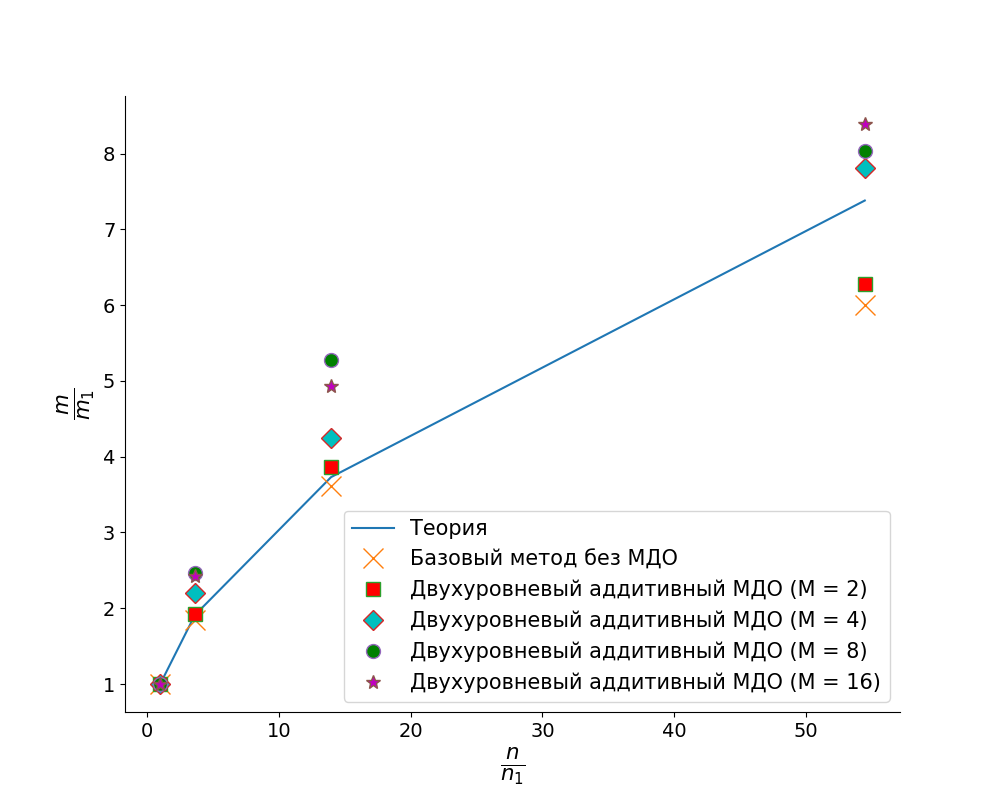
\includegraphics[scale=0.5]{../results/\area/\task/core/iters_cg.png}}
\caption{График отношений количества итераций}
\label{fig:task_\taskNum_iters_cg}
\end{figure}
\begin{figure}[H]
\center{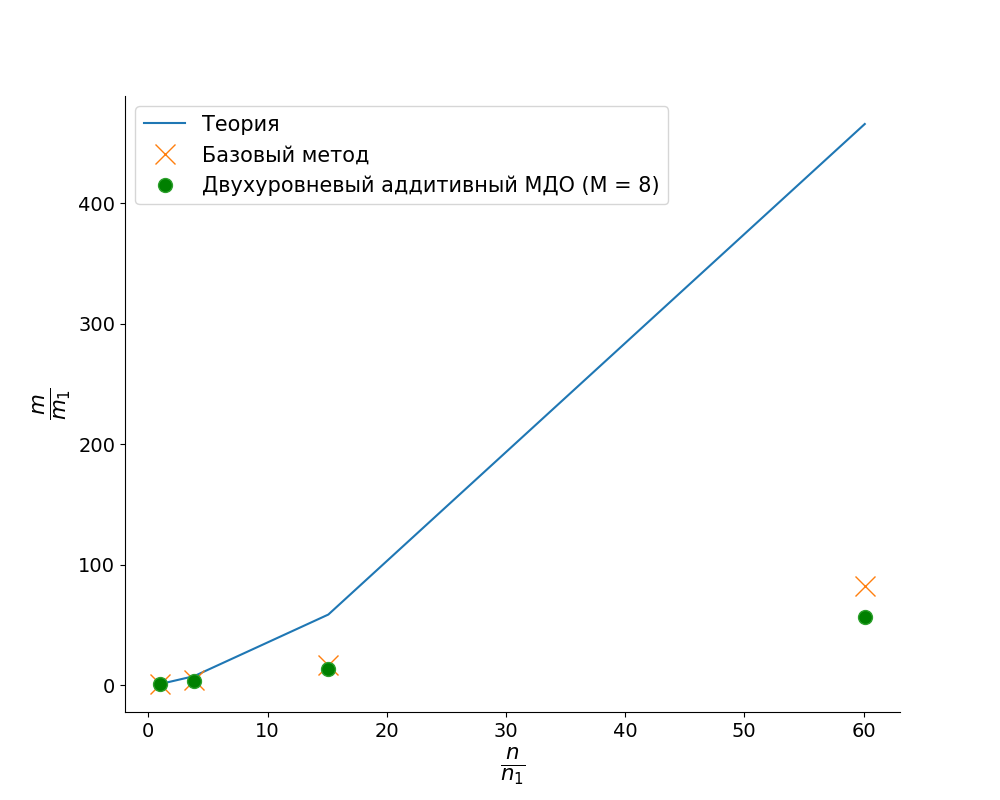
\includegraphics[scale=0.5]{../results/\area/\task/core/time_cg.png}}
\caption{График отношений временных затрат}
\label{fig:task_\taskNum_time_cg}
\end{figure}

\newpage

\begin{center}
\section*{\centering ЗАКЛЮЧЕНИЕ}
\end{center}
\addcontentsline{toc}{section}{ЗАКЛЮЧЕНИЕ}

Цели и задачи, поставленные в магистерской работе, выполнены. Изучены математические модели для задач деформирования упругих тел, исследованы мультипликативный, аддитивный и двухуровневый аддитивный методы Шварца. Данные методы реализованы в виде программы, написанной на языке Python. Проведены серии расчётов для четырёх тестовых задач. Выполнено исследование сходимости путём сравнения количества итераций для мультипликативного, аддитивного и двухуровневого аддитивного методов Шварца, изучена скорость роста итераций и временных затрат при решении задачи методом сопряженных градиентов.

Результаты, полученные при решении ряда тестовых задач, показывают, что двухуровневый аддитивный метод Шварца выигрывает у мультипликативного и аддитивного методов Шварца по нескольким параметрам: во-первых, локальные задачи в каждой из подобластей решаются независимо друг от друга, количество итераций не зависит практически ни от изменения шага сетки, ни от изменения количества подобластей, на которое разбивается исходная область.

Анализ результатов количества итераций и временных затрат при решении задачи методом сопряженных градиентов показал, что скорости роста количества итераций для базового случая решения задачи без методов декомпозиции области и двухуровневого аддитивного метода Шварца практически не отличаются друг от друга, а скорость роста временных затрат при решении задачи двухуровневым аддитивным методом Шварца меньше, чем при решении задачи базовым методом без применения методом декомпозиции области.

\renewcommand{\refname}{\centering\textbf\selectfont\large СПИСОК ИСПОЛЬЗОВАННЫХ ИСТОЧНИКОВ} 
\newpage
\addcontentsline{toc}{section}{СПИСОК ИСПОЛЬЗОВАННЫХ ИСТОЧНИКОВ}
\begin{thebibliography}{9}
\bibitem{1}  Зарубин В.С., Кувыркин Г.Н. Математические модели механики и электродинамики сплошной среды. - М. МГТУ им. Н.Э.Баумана, 2008.-512 с.
\bibitem{2}  Феодосьев В.И. Сопротивление материалов. - М. МГТУ им. Н.Э.Баумана, 2010. 591 с.
\bibitem{3}  Сагдеева, Ю.А. Введение в метод конечных элементов: метод.пособие/Ю.А.Сагдеева,С.П.Копысов,А.К.Новиков.-Ижевск:Изд-во "Удмуртский университет".2011. 44с
\bibitem{4}  Погорелов В.И. Строительная механика тонкостенных конструкций.-СПб.: БХВ-Петербург,2007.-528 с.:ил.
\bibitem{5}  Алексеев Г.В. Численные методы математической физики.Введение в метод конечных элементов.-Владивосток:Изд-во "Институт прикладной математики ДВО РАН".1999. 125с.
\bibitem{6}  Князева А.Г. Теплофизические основы современных методов металлообработки.-Томск:Изд-во "Томский политехнический университет".2009.-48 с.
\bibitem{7}  Князева А.Г. Различные варианты метода прогонки.-Томск:Изд-во "Томский политехнический университет".2006.-8 с.
\bibitem{8}  Галанин М.П.,Савенков Е.Б. Методы численного анализа математических моделей. - М. МГТУ им. Н.Э.Баумана, 2010.-591 с.
\bibitem{9}  Малинин Н. Н. Прикладная теория пластичности и ползучести. Учебник для студентов вузов. Изд. 2-е, перераб. и доп. М., «Машиностроение», 1975, 400 с. с ил.
\bibitem{10} Писаренко Г. С., Можаровский Н. С. Уравнения и краевые задачи теории пластичности и ползучести. Справочное пособие— Киев: Наук. думка, 1981.— 496 с.
\bibitem{11} Митчелл Э., Уэйт Р. Метод конечных элементов для уравнений с частными производными. М.: Мир, 1981. - 216 с.
\bibitem{12} Zienkiewicz O.C., Taylor R.L., Fox D.D. The finite element method for solid and structural mechanics, 5th Edition. - Elsevier, 2014. — 657 p
\bibitem{13} Глизнуцина П.В., Лукин В.В., Родин А.С. Реализация условия механического контакта упругих тел в рамках МКЭ при различном выборе базисных функций: одномерный случай // Препринты ИПМ им. М.В.Келдыша. 2015. № 90. 25 с.
\bibitem{14} Станкевич И.В., Волков С.С. Алгоритмы решения краевых задач МДТТ с учётом деформации ползучести. Математика и математическое моделирование. 2018;(1):1-14.

\end{thebibliography}


\end{document}
